%
\section{Example}
\label{sec_ex}
In this section, we illustrate the proposed STC approach with a numerical example from the literature. We consider the single link robot arm example from \cite{postoyan2014tracking}. The plant is given by 
\begin{equation*}
	\begin{split}
		x_{p,1}&= x_{p,2}\\
		x_{p,2}&= -a\sin(x_{p,1}) + b\hat{u}\\
		y&=x_{p,1}
	\end{split}	
\end{equation*}
and the static state-feedback controller by \linebreak
%
	$u = b^{-1}\left(a\sin(x_{o,1})-x_{o,1}-x_{o,2}\right).$
%
%
We consider an observer given by 
\begin{equation*}
	\begin{split}
		x_{o,1} &= x_{o,2} + \theta_1\left(y-x_{o,1}\right)\\
		x_{o,2} &= -a\sin(x_{o,1}) +b\hat{u} + \theta_2\left(y-x_{o,1}\right)
	\end{split}
\end{equation*}
for $\theta_1,\theta_2\in\R$. We define $x_p = \begin{bmatrix}
	x_{p,1} & x_{p,2}
\end{bmatrix}^\top$, $e = \begin{bmatrix}
	e_1 & e_2
\end{bmatrix}^\top = \begin{bmatrix}
	\hat{x}_{o,1} - x_{p,1} & \hat{x}_{o,2} - x_{p,2}
\end{bmatrix}^\top$
and $e_o = \begin{bmatrix}
	e_{o,1} & e_{o,2}
\end{bmatrix}^\top = \linebreak \begin{bmatrix}
	{x}_{o,1} - x_{p,1} & {x}_{o,2} - x_{p,2}
\end{bmatrix}^\top$.

Note again that Assumption~\ref{asum_hybrid_lyap} is identical as for the state-feedback case and can thus be verified as in state-feedback case based on linear matrix inequalities. Details on the verification procedure for the considered example are omitted for brevity but can be found in \cite[Section VI.A]{hertneck21robust_arxiv}.
%
%
Using 
\begin{equation*}
	\begin{split}
		&-a\left(\sin(x_{p,1}) - \sin(x_{o,1})\right)\\
%
		=&2a\cos\left(\frac{2x_{p,1}+e_{o,1}}{2}\right) \sin\left(-\frac{e_{o,1}}{2}\right) = \tilde{a} e_{o,1}
	\end{split}
\end{equation*}
for a varying parameter $\tilde{a}\in\left[-a,a\right]$, the dynamics of the observer error can be written as
%
	$\dot{e}_o = \begin{bmatrix}
		-\theta_1 & 1\\
		-\theta_2+\tilde{a} & 0
	\end{bmatrix} e_o$
%
and it can be easily verified that Assumption~\ref{as_obs_er} holds if $\theta_1 > 0$ and $\theta_2 + \tilde{a} > 0$ for all $\tilde{a}\in\left[-a,a\right]$. 
%
Subsequently, we consider $a = \frac{9.81}{2}$ and $b=2$. Using the approach from \cite[Section~VI.A]{hertneck21robust_arxiv}, we have computed $n_\tpar = 23$ different parameter sets that satisfy Assumption~\ref{asum_hybrid_lyap} with $\epsilon_i \in \left[-20,0.01\right]$. Moreover, we have chosen $\theta_1 = \theta_2 = 10$. The maximum sampling interval, for which UGAS can be guaranteed for periodic sampling, is $t_{\min} = \SI{0.175}{\second}$. 

To demonstrate our approach, we compare the required number of transmissions for the proposed STC mechanism  for 1000 randomly selected initial conditions to the number of transmissions that are needed for periodic sampling with stability guarantees. 
%
The initial conditions for $x_p$ and $x_o$ where drawn uniformly from 
%
$	\begin{bmatrix}
		x_{p,1}(0,0)& x_{p,2}(0,0)& x_{o,1}(0,0)& x_{o,2}(0,0)
	\end{bmatrix}\in\left[-10,10\right]^4.$
%
 We consider $n_\eta = 15$ and $\eta_i(0,0) = V(x_o(0,0))$ for $i\in\left\lbrace 1,\dots,n_\eta \right\rbrace$. In the first $\SI{10}{\second}$, the proposed STC mechanism requires on average 29.8 transmissions. In comparison, for periodic sampling 56 transmissions are needed for the same time span. For trajectories with a duration of $\SI{50}{\second}$ and the same initial conditions, the proposed STC mechanism requires on average 92.4 samples whilst 282 transmissions are needed for periodic sampling, leading to reduction of the required number of transmissions by factor $\frac{1}{3}$ for the proposed STC approach. 
%
For the considered example, the amount of reduction is larger if a larger time span is considered. A reason for that is that the observer state $x_o$ is used to determine transmission times instead of the plant state $x_p$. It can therefore happen that the value of $V(x_o)$, i.e., of the Lyapunov function for the observer state increases significantly at the beginning as the observer state converges, leading to frequent transmissions at the beginning. An exemplary trajectory where this occurs is given in Figure~\ref{fig_states}. The respective transmission intervals are given in Figure~\ref{fig_inters}.
%
%
To compensate the initial increase of the Lyapunov function, the initial values for $\eta$ could be chosen differently at the cost of reduced convergence speed.


\begin{figure}
	\centering
		%
%
%
%
%
%
%
\definecolor{mycolor1}{rgb}{0.00000,0.44700,0.74100}%
\definecolor{mycolor2}{rgb}{0.85000,0.32500,0.09800}%
%
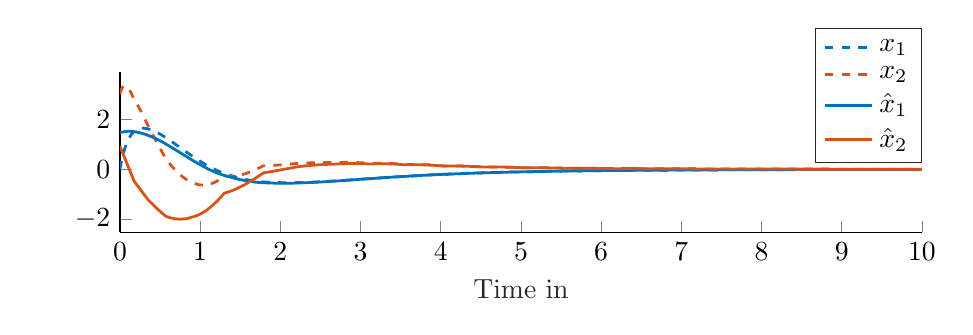
\begin{tikzpicture}

\begin{axis}[%
width=.84\linewidth,
height=.8in,
at={(0in,0in)},
scale only axis,
xmin=0,
xmax=10.0,
xlabel style={font=\color{white!15!black}},
xlabel={Time in \SI{}{\second}},
ylabel style={font=\color{white}},
ylabel={Transm. int},
axis background/.style={fill=white},
%
%
axis x line*=bottom,
axis y line*=left,
legend style={legend cell align=left, align=left, draw=white!15!black,at={(1,1.28)}}
]
\addplot [color=mycolor1, dashed, line width=1.0pt]
  table[row sep=crcr]{%
0	0.00114374817344887\\
3.24858708220529e-06	0.00120120666064957\\
6.49717416441059e-06	0.00125866350156172\\
9.74576124661588e-06	0.00131611869622736\\
1.29943483288212e-05	0.00137357224468855\\
2.92372837398476e-05	0.00166081529539931\\
4.54802191508741e-05	0.00194801719730559\\
6.17231545619006e-05	0.00223517795566245\\
7.7966089972927e-05	0.00252229757572424\\
0.000159180767028059	0.00395727878546081\\
0.000240395444083192	0.00539123232557297\\
0.000321610121138324	0.00682415885207123\\
0.000402824798193456	0.00825605902053143\\
0.000808898183469118	0.0154001874073762\\
0.00121497156874478	0.0225187549299731\\
0.00162104495402044	0.0296118430480991\\
0.0020271183392961	0.0366795329532868\\
0.00405748526567441	0.0716398334305637\\
0.00608785219205272	0.105977203872892\\
0.00811821911843103	0.139701496692303\\
0.0101485860448093	0.172822406919171\\
0.0145800306643543	0.243061938254582\\
0.0190114752838992	0.310568968421262\\
0.0234429199034442	0.375436762673016\\
0.0278743645229891	0.437755502004517\\
0.0323058091425341	0.497612276861365\\
0.036737253762079	0.555091020750227\\
0.041168698381624	0.610272872285892\\
0.0456001430011689	0.663236311713635\\
0.0500315876207138	0.714057145161778\\
0.0544630322402588	0.762808423936637\\
0.0588944768598037	0.809560757043587\\
0.0633259214793487	0.854382426514995\\
0.0677573660988936	0.897339368933337\\
0.0721888107184386	0.938495094408023\\
0.0766202553379835	0.977910962401909\\
0.0810516999575285	1.0156462822043\\
0.0854831445770734	1.05175829517305\\
0.0899145891966183	1.08630210035482\\
0.0943460338161633	1.11933090016385\\
0.0987774784357082	1.1508960893101\\
0.103208923055253	1.18104723921345\\
0.107640367674798	1.20983203293045\\
0.112071812294343	1.23729648419436\\
0.116503256913888	1.26348501653358\\
0.120934701533433	1.28844045024008\\
0.125366146152978	1.31220394695826\\
0.129797590772523	1.33481520433387\\
0.134229035392068	1.35631252633562\\
0.138660480011613	1.37673281265451\\
0.143091924631158	1.39611151223176\\
0.147523369250703	1.41448279535762\\
0.151954813870248	1.43187961592769\\
0.156386258489793	1.4483337029544\\
0.160817703109337	1.46387552191194\\
0.165249147728882	1.47853442606516\\
0.169680592348427	1.49233871130924\\
0.17157489045677	1.49798560873988\\
0.173469188565113	1.50348339294692\\
0.175363486673455	1.50883409700587\\
0.177257784781798	1.5140397212649\\
0.177257784781798	1.5140397212649\\
0.181689229401343	1.52569749297194\\
0.186120674020888	1.53666760262376\\
0.190552118640433	1.54697361078621\\
0.194983563259978	1.55663821786737\\
0.199415007879523	1.56568325940858\\
0.203846452499067	1.57412968189719\\
0.208277897118612	1.58199765130151\\
0.212709341738157	1.58930659260253\\
0.217140786357702	1.59607518603782\\
0.221572230977247	1.60232134699525\\
0.226003675596792	1.60806231986849\\
0.230435120216337	1.613314712288\\
0.234866564835882	1.61809449212148\\
0.239298009455427	1.62241697074483\\
0.243729454074972	1.62629688396611\\
0.248160898694517	1.62974842157704\\
0.252592343314062	1.63278522495495\\
0.257023787933607	1.63542037313039\\
0.261455232553152	1.63766645239158\\
0.265886677172697	1.63953558173199\\
0.270318121792242	1.64103941093185\\
0.274749566411787	1.64218910894514\\
0.279181011031332	1.64299542364759\\
0.283612455650877	1.64346870370535\\
0.288043900270421	1.64361889703997\\
0.292475344889966	1.64345554114217\\
0.296906789509511	1.64298781427516\\
0.301338234129056	1.64222455423631\\
0.305769678748601	1.64117425713001\\
0.310201123368146	1.63984506928468\\
0.314632567987691	1.63824483107544\\
0.319064012607236	1.63638109299875\\
0.323495457226781	1.6342611146932\\
0.327926901846326	1.63189185819264\\
0.332358346465871	1.62928002539249\\
0.336789791085416	1.62643207180827\\
0.341221235704961	1.62335420579631\\
0.345652680324506	1.62005238292155\\
0.350084124944051	1.61653233796366\\
0.354515569563596	1.61279959668396\\
0.354515569563596	1.61279959668396\\
0.360000487484141	1.60790748425292\\
0.365485405404687	1.60273653277488\\
0.370970323325232	1.59729593294547\\
0.376455241245778	1.59159447370169\\
0.381940159166324	1.585640539306\\
0.387425077086869	1.57944209662452\\
0.392909995007415	1.57300676249775\\
0.398394912927961	1.56634182752215\\
0.403879830848506	1.55945425374808\\
0.409364748769052	1.55235066442814\\
0.414849666689598	1.54503739930527\\
0.420334584610143	1.53752053415742\\
0.425819502530689	1.52980587897988\\
0.431304420451235	1.52189896971376\\
0.43678933837178	1.51380511361426\\
0.442274256292326	1.50552940531299\\
0.447759174212871	1.49707672538116\\
0.453244092133417	1.48845173364335\\
0.458729010053963	1.47965890641033\\
0.464213927974508	1.47070254968205\\
0.469698845895054	1.46158679800833\\
0.4751837638156	1.45231560906913\\
0.480668681736145	1.44289279424027\\
0.486153599656691	1.43332202944944\\
0.491638517577237	1.42360685426752\\
0.497123435497782	1.4137506674973\\
0.502608353418328	1.40375675227731\\
0.508093271338873	1.39362828501156\\
0.513578189259419	1.38336833463722\\
0.519063107179965	1.37297985901282\\
0.52454802510051	1.36246572554741\\
0.530032943021056	1.35182871854851\\
0.535517860941602	1.34107153862211\\
0.541002778862147	1.33019679969091\\
0.546487696782693	1.31920704595585\\
0.551972614703239	1.30810475794391\\
0.557457532623784	1.2968923520046\\
0.56294245054433	1.28557217782058\\
0.568427368464875	1.27414653236045\\
0.573912286385421	1.26261766485605\\
0.573912286385421	1.26261766485605\\
0.578852481799184	1.25216460885918\\
0.583792677212947	1.24166593246526\\
0.58873287262671	1.23112318117265\\
0.593673068040473	1.22053787534196\\
0.601647225060544	1.20336574630449\\
0.609621382080615	1.18609277748384\\
0.617595539100685	1.16872497052946\\
0.625569696120756	1.15126821544123\\
0.633543853140827	1.13372828475883\\
0.641518010160898	1.11611081923325\\
0.649492167180969	1.09842137647239\\
0.65746632420104	1.08066544612188\\
0.665440481221111	1.06284844479317\\
0.673414638241182	1.04497570372835\\
0.681388795261253	1.02705250522358\\
0.689362952281324	1.00908409380994\\
0.697337109301394	0.991075671659493\\
0.705311266321465	0.973032387623454\\
0.713285423341536	0.954959364424775\\
0.721259580361607	0.93686170678239\\
0.729233737381678	0.918744497121811\\
0.737207894401749	0.900612785564934\\
0.74518205142182	0.882471610124228\\
0.753156208441891	0.864326002481455\\
0.761130365461962	0.846180983895458\\
0.769104522482033	0.828041555871604\\
0.777078679502104	0.80991271503289\\
0.785052836522175	0.791799457094944\\
0.793026993542245	0.773706772913753\\
0.801001150562316	0.755639639674855\\
0.808975307582387	0.737603031708405\\
0.816949464602458	0.719601923078859\\
0.824923621622529	0.701641283752636\\
0.8328977786426	0.683726071230124\\
0.840871935662671	0.665861238271989\\
0.848846092682742	0.648051734431609\\
0.856820249702813	0.630302502349431\\
0.864794406722884	0.612618469810324\\
0.872768563742955	0.595004555127104\\
0.880742720763026	0.577465667876942\\
0.883776682369333	0.570813297076702\\
0.886810643975641	0.564172765114322\\
0.889844605581949	0.557544340687991\\
0.892878567188257	0.550928292169526\\
0.892878567188257	0.550928292169526\\
0.902939255666085	0.529057364313897\\
0.912999944143914	0.507287387624924\\
0.923060632621742	0.485628079586304\\
0.93312132109957	0.464089131236303\\
0.94335809302201	0.442306709503388\\
0.953594864944451	0.420668997769727\\
0.963831636866891	0.399186046533689\\
0.974068408789331	0.377867849935513\\
0.984305180711772	0.356724334660571\\
0.994541952634212	0.335765338195269\\
1.00477872455665	0.315000613573458\\
1.01501549647909	0.294439827109869\\
1.02525226840153	0.274092548572838\\
1.03548904032397	0.253968232167559\\
1.04572581224641	0.234076218530483\\
1.05596258416885	0.214425731905755\\
1.0661993560913	0.195025871724912\\
1.07643612801374	0.175885596545906\\
1.08667289993618	0.157013724404452\\
1.09690967185862	0.138418929864509\\
1.10714644378106	0.120109737088871\\
1.1173832157035	0.102094506855919\\
1.12761998762594	0.0843814360384144\\
1.13785675954838	0.0669785548281141\\
1.14809353147082	0.0498937213108546\\
1.15833030339326	0.0331346115455753\\
1.1685670753157	0.0167087186731655\\
1.17880384723814	0.000623350501493425\\
1.18904061916058	-0.0151143744755933\\
1.19927739108302	-0.0304975340966184\\
1.20951416300546	-0.0455194034987903\\
1.2197509349279	-0.0601734570816575\\
1.22998770685034	-0.0744533711723718\\
1.24022447877278	-0.0883530284320397\\
1.25046125069522	-0.101866518756283\\
1.26069802261766	-0.114988140771908\\
1.27111087798472	-0.12792776667731\\
1.28152373335177	-0.140450692371186\\
1.29193658871882	-0.152551592344322\\
1.30234944408587	-0.164225370558407\\
1.30234944408587	-0.164225370558407\\
1.3098468225062	-0.172444608607434\\
1.31734420092653	-0.180600530195094\\
1.32484157934685	-0.188691389307528\\
1.33233895776718	-0.196715458630009\\
1.34454334819472	-0.209629946630653\\
1.35674773862227	-0.222355674367174\\
1.36895212904981	-0.234885520907739\\
1.38115651947735	-0.247212509637471\\
1.39336090990489	-0.25932981017053\\
1.40556530033244	-0.271230738983149\\
1.41776969075998	-0.282908767142256\\
1.42997408118752	-0.294357524582748\\
1.44217847161506	-0.305570800916315\\
1.45438286204261	-0.316542544218242\\
1.46658725247015	-0.327266869337502\\
1.47879164289769	-0.337738061879983\\
1.49099603332523	-0.347950578120951\\
1.50320042375278	-0.357899042361032\\
1.51540481418032	-0.367578255196023\\
1.52760920460786	-0.376983197067276\\
1.5398135950354	-0.386109027482972\\
1.55201798546295	-0.394951081351497\\
1.56422237589049	-0.403504876831162\\
1.57642676631803	-0.411766118390252\\
1.58863115674557	-0.41973069553822\\
1.60083554717312	-0.427394678533281\\
1.61303993760066	-0.434754325598691\\
1.6252443280282	-0.441806085490171\\
1.63744871845574	-0.448546595928232\\
1.64965310888329	-0.454972679055274\\
1.66185749931083	-0.461081347913343\\
1.67406188973837	-0.466869808550023\\
1.68626628016591	-0.472335458326046\\
1.69847067059345	-0.477475881463331\\
1.710675061021	-0.482288854742015\\
1.72287945144854	-0.486772349191066\\
1.73508384187608	-0.490924528421399\\
1.74728823230362	-0.494743744560588\\
1.75949262273117	-0.498228543154374\\
1.77169701315871	-0.501377664488704\\
1.77640402516593	-0.502502292166475\\
1.78111103717314	-0.503576773188985\\
1.78581804918036	-0.50460105821478\\
1.79052506118757	-0.50557510218453\\
1.79052506118757	-0.50557510218453\\
1.80162616690817	-0.507774900889518\\
1.81272727262876	-0.509898118356597\\
1.82382837834935	-0.511944284767475\\
1.83492948406995	-0.513912957139501\\
1.84603058979054	-0.515803718997884\\
1.85713169551113	-0.517616179475676\\
1.86823280123173	-0.519349975803809\\
1.87933390695232	-0.521004774113346\\
1.89043501267292	-0.522580269151458\\
1.90153611839351	-0.524076183525248\\
1.9126372241141	-0.525492269705408\\
1.9237383298347	-0.526828310662161\\
1.93483943555529	-0.528084119616111\\
1.94594054127588	-0.529259539408586\\
1.95704164699648	-0.530354444092446\\
1.96814275271707	-0.531368739423107\\
1.97924385843767	-0.532302362638214\\
1.99034496415826	-0.533155281942404\\
2.00144606987885	-0.533927497737098\\
2.01254717559945	-0.534619042981844\\
2.02364828132004	-0.535229982998497\\
2.03474938704063	-0.535760415061514\\
2.04585049276123	-0.53621046930334\\
2.05695159848182	-0.536580308956936\\
2.06805270420241	-0.536870130181157\\
2.07915380992301	-0.537080161749465\\
2.0902549156436	-0.537210665656838\\
2.1013560213642	-0.537261937251213\\
2.11245712708479	-0.537234305077263\\
2.12355823280538	-0.537128130657227\\
2.13465933852598	-0.536943808817794\\
2.14576044424657	-0.536681767715905\\
2.15686154996716	-0.536342468698333\\
2.16796265568776	-0.535926406168544\\
2.17906376140835	-0.535434107646756\\
2.19016486712894	-0.534866133693936\\
2.20126597284954	-0.534223077784598\\
2.21236707857013	-0.533505566253428\\
2.22346818429073	-0.532714258098158\\
2.23456929001132	-0.531849844804449\\
2.23456929001132	-0.531849844804449\\
2.2453378327922	-0.530952752945335\\
2.25610637557309	-0.530009424079574\\
2.26687491835397	-0.529020560769699\\
2.27764346113485	-0.527986883234206\\
2.28841200391574	-0.526909129267683\\
2.29918054669662	-0.525788054311936\\
2.30994908947751	-0.524624430865583\\
2.32071763225839	-0.523419048183662\\
2.33148617503927	-0.522172712201674\\
2.34225471782016	-0.520886245640509\\
2.35302326060104	-0.519560487258712\\
2.36379180338193	-0.518196291492299\\
2.37456034616281	-0.516794528380728\\
2.38532888894369	-0.515356083699812\\
2.39609743172458	-0.513881858068988\\
2.40686597450546	-0.512372766535398\\
2.41763451728634	-0.510829738500224\\
2.42840306006723	-0.509253717874401\\
2.43917160284811	-0.507645662052031\\
2.449940145629	-0.50600654144261\\
2.46070868840988	-0.504337339396524\\
2.47147723119076	-0.50263905237891\\
2.48224577397165	-0.500912688819878\\
2.49301431675253	-0.499159268598805\\
2.50378285953341	-0.497379822968129\\
2.5145514023143	-0.495575394741178\\
2.52531994509518	-0.493747037029911\\
2.53608848787607	-0.49189581268537\\
2.54685703065695	-0.490022794219263\\
2.55762557343783	-0.488129064002016\\
2.56839411621872	-0.486215712899137\\
2.5791626589996	-0.484283839672232\\
2.58993120178049	-0.482334550898165\\
2.60069974456137	-0.480368961174057\\
2.61146828734225	-0.478388191663972\\
2.62223683012314	-0.476393369465306\\
2.63300537290402	-0.474385627525615\\
2.6437739156849	-0.4723661048517\\
2.65454245846579	-0.470335944979114\\
2.66531100124667	-0.468296295309122\\
2.66531100124667	-0.468296295309122\\
2.6764092766314	-0.466174035235325\\
2.68750755201612	-0.464021302556612\\
2.69860582740085	-0.46183938313607\\
2.70970410278557	-0.459629577126379\\
2.7208023781703	-0.457393198858835\\
2.73190065355502	-0.455131577105014\\
2.74299892893975	-0.452846053188263\\
2.75409720432447	-0.450537980155989\\
2.7651954797092	-0.448208722662841\\
2.77629375509392	-0.445859657238519\\
2.78739203047865	-0.443492170282281\\
2.79849030586338	-0.44110765718836\\
2.8095885812481	-0.438707522224196\\
2.82068685663283	-0.43629317880171\\
2.83178513201755	-0.433866047368349\\
2.84288340740228	-0.431427554491914\\
2.853981682787	-0.428979132735018\\
2.86507995817173	-0.426522220927414\\
2.87617823355645	-0.4240582619698\\
2.88727650894118	-0.421588701885439\\
2.8983747843259	-0.419114989692303\\
2.90947305971063	-0.416638577674392\\
2.92057133509535	-0.414160919116852\\
2.93166961048008	-0.411683467332712\\
2.9427678858648	-0.409207675534436\\
2.95386616124953	-0.406734997102589\\
2.96496443663425	-0.404266883272752\\
2.97606271201898	-0.401804782146488\\
2.9871609874037	-0.399350138564298\\
2.99825926278843	-0.396904394370359\\
3.00935753817315	-0.394468986073293\\
3.02045581355788	-0.392045343851126\\
3.03155408894261	-0.389634891427822\\
3.04265236432733	-0.38723904633319\\
3.05375063971206	-0.384859217560739\\
3.06484891509678	-0.382496804576866\\
3.07594719048151	-0.380153197203292\\
3.08704546586623	-0.3778297758715\\
3.09814374125096	-0.375527909301724\\
3.10924201663568	-0.373248953526895\\
3.10924201663568	-0.373248953526895\\
3.12034312235628	-0.370971660698577\\
3.13144422807687	-0.368675939762909\\
3.14254533379746	-0.366363144819437\\
3.15364643951806	-0.364034639105795\\
3.16474754523865	-0.361691794858372\\
3.17584865095924	-0.359335993556275\\
3.18694975667984	-0.356968623749905\\
3.19805086240043	-0.354591080116497\\
3.20915196812102	-0.352204763318997\\
3.22025307384162	-0.349811080253868\\
3.23135417956221	-0.347411441802619\\
3.24245528528281	-0.345007261858601\\
3.2535563910034	-0.342599957186\\
3.26465749672399	-0.340190947670106\\
3.27575860244459	-0.337781654010117\\
3.28685970816518	-0.335373496725638\\
3.29796081388577	-0.332967896017806\\
3.30906191960637	-0.330566272020798\\
3.32016302532696	-0.328170042456332\\
3.33126413104756	-0.325780621629109\\
3.34236523676815	-0.323399420292203\\
3.35346634248874	-0.321027845898749\\
3.36456744820934	-0.318667300240168\\
3.37566855392993	-0.316319178440384\\
3.38676965965052	-0.313984868827695\\
3.39787076537112	-0.311665753185731\\
3.40897187109171	-0.309363204398567\\
3.4200729768123	-0.307078585453956\\
3.4311740825329	-0.304813249323909\\
3.44227518825349	-0.302568539214145\\
3.45337629397409	-0.300345786239935\\
3.46447739969468	-0.298146308448799\\
3.47557850541527	-0.295971410711997\\
3.48667961113587	-0.293822384971754\\
3.49778071685646	-0.291700507971937\\
3.50888182257705	-0.289607040310682\\
3.51998292829765	-0.287543226344901\\
3.53108403401824	-0.285510294434591\\
3.54218513973884	-0.283509454752267\\
3.55328624545943	-0.281541898375842\\
3.55328624545943	-0.281541898375842\\
3.56528776808197	-0.279426040731817\\
3.57728929070451	-0.277296913755646\\
3.58929081332705	-0.275156000604952\\
3.60129233594959	-0.273004791833607\\
3.61329385857213	-0.27084478519356\\
3.62529538119467	-0.268677485922878\\
3.63729690381721	-0.266504403863544\\
3.64929842643975	-0.264327052206535\\
3.6612999490623	-0.262146947299545\\
3.67330147168484	-0.259965608947335\\
3.68530299430738	-0.257784557455303\\
3.69730451692992	-0.255605312351611\\
3.70930603955246	-0.253429392203686\\
3.721307562175	-0.251258314928734\\
3.73330908479754	-0.249093594794802\\
3.74531060742008	-0.246936741134134\\
3.75731213004262	-0.244789258171385\\
3.76931365266516	-0.242652645342185\\
3.7813151752877	-0.240528394285189\\
3.79331669791024	-0.238417987561452\\
3.80531822053278	-0.236322898497247\\
3.81731974315532	-0.234244591508618\\
3.82932126577786	-0.232184519118997\\
3.84132278840041	-0.230144120699708\\
3.85332431102295	-0.228124822330172\\
3.86532583364549	-0.226128037126406\\
3.87732735626803	-0.22415516231921\\
3.88932887889057	-0.222207578030945\\
3.90133040151311	-0.220286647155736\\
3.91333192413565	-0.218393715689826\\
3.92533344675819	-0.216530109905152\\
3.93733496938073	-0.214697135177291\\
3.94933649200327	-0.212896075888022\\
3.96133801462581	-0.211128195755368\\
3.97333953724835	-0.209394735136572\\
3.98534105987089	-0.207696909921627\\
3.99734258249343	-0.20603591146021\\
4.00934410511598	-0.204412906889154\\
4.02134562773852	-0.202829036597468\\
4.03334715036106	-0.201285413199121\\
4.03334715036106	-0.201285413199121\\
4.04562392660128	-0.199722031915939\\
4.05790070284151	-0.198148794945395\\
4.07017747908174	-0.196566859903969\\
4.08245425532196	-0.194977390072279\\
4.09473103156219	-0.193381554223076\\
4.10700780780241	-0.191780526846378\\
4.11928458404264	-0.190175485753631\\
4.13156136028287	-0.188567611032037\\
4.14383813652309	-0.186958084881449\\
4.15611491276332	-0.185348091855527\\
4.16839168900355	-0.183738816410413\\
4.18066846524377	-0.182131441844132\\
4.192945241484	-0.180527150144634\\
4.20522201772422	-0.178927122244626\\
4.21749879396445	-0.177332535543221\\
4.22977557020468	-0.175744562842921\\
4.2420523464449	-0.17416437221097\\
4.25432912268513	-0.172593127245448\\
4.26660589892536	-0.171031984599205\\
4.27888267516558	-0.169482092927163\\
4.29115945140581	-0.167944592763039\\
4.30343622764604	-0.166420616794225\\
4.31571300388626	-0.164911287417682\\
4.32798978012649	-0.163417715710338\\
4.34026655636672	-0.161941001323092\\
4.35254333260694	-0.160482232761919\\
4.36482010884717	-0.159042485005322\\
4.37709688508739	-0.157622818510443\\
4.38937366132762	-0.156224279126034\\
4.40165043756785	-0.154847898377191\\
4.41392721380807	-0.153494691173386\\
4.4262039900483	-0.15216565486256\\
4.43848076628853	-0.150861769164529\\
4.45075754252875	-0.149583996456629\\
4.46303431876898	-0.148333279600423\\
4.47531109500921	-0.147110541055476\\
4.48758787124943	-0.145916682834388\\
4.49986464748966	-0.144752586786577\\
4.51214142372988	-0.143619112570355\\
4.52441819997011	-0.14251709683739\\
4.52441819997011	-0.14251709683739\\
4.53747174027572	-0.141357970398869\\
4.55052528058133	-0.140190691398325\\
4.56357882088695	-0.139016234702613\\
4.57663236119256	-0.137835580467598\\
4.58968590149817	-0.136649713965863\\
4.60273944180378	-0.135459625793814\\
4.61579298210939	-0.13426630956998\\
4.62884652241501	-0.133070760926459\\
4.64190006272062	-0.131873977348382\\
4.65495360302623	-0.130676958401392\\
4.66800714333184	-0.129480703374561\\
4.68106068363745	-0.128286210258319\\
4.69411422394307	-0.127094475597957\\
4.70716776424868	-0.125906494738691\\
4.72022130455429	-0.124723259444534\\
4.7332748448599	-0.123545756876387\\
4.74632838516551	-0.122374969461729\\
4.75938192547113	-0.121211875154296\\
4.77243546577674	-0.120057445060815\\
4.78548900608235	-0.118912642433056\\
4.79854254638796	-0.11777842255566\\
4.81159608669357	-0.116655733017302\\
4.82464962699919	-0.115545511377308\\
4.8377031673048	-0.114448684185328\\
4.85075670761041	-0.113366166889052\\
4.86381024791602	-0.11229886411358\\
4.87686378822163	-0.111247667399548\\
4.88991732852725	-0.110213454263772\\
4.90297086883286	-0.109197088128323\\
4.91602440913847	-0.108199418604736\\
4.92907794944408	-0.107221279334374\\
4.94213148974969	-0.106263487102897\\
4.95518503005531	-0.105326841791849\\
4.96823857036092	-0.104412126664259\\
4.98129211066653	-0.103520106336658\\
4.99434565097214	-0.102651525959474\\
5.00739919127775	-0.101807111192004\\
5.02045273158337	-0.100987568485882\\
5.03350627188898	-0.100193583216385\\
5.04655981219459	-0.0994258189400062\\
5.04655981219459	-0.0994258189400062\\
5.06042820686669	-0.0986204276453921\\
5.07429660153879	-0.097807828655519\\
5.08816499621089	-0.0969887891147167\\
5.10203339088299	-0.096164081636115\\
5.11590178555509	-0.0953344841380031\\
5.12977018022719	-0.09450078001769\\
5.14363857489929	-0.0936637560998523\\
5.15750696957139	-0.0928242017310563\\
5.17137536424349	-0.0919829086284172\\
5.18524375891559	-0.091140671076311\\
5.19911215358769	-0.0902982838129104\\
5.21298054825979	-0.0894565411087851\\
5.22684894293189	-0.0886162366301976\\
5.24071733760399	-0.087778163655782\\
5.25458573227609	-0.0869431129330737\\
5.26845412694819	-0.0861118717550877\\
5.28232252162029	-0.0852852238403896\\
5.29619091629239	-0.0844639495665932\\
5.31005931096449	-0.0836488238292577\\
5.32392770563659	-0.0828406151304239\\
5.33779610030869	-0.0820400854773651\\
5.35166449498079	-0.0812479906295284\\
5.36553288965289	-0.0804650779922265\\
5.379401284325	-0.0796920857309717\\
5.3932696789971	-0.0789297426905383\\
5.40713807366919	-0.0781787686517852\\
5.42100646834129	-0.0774398722921097\\
5.4348748630134	-0.0767137503390549\\
5.4487432576855	-0.0760010875110119\\
5.4626116523576	-0.0753025567802149\\
5.4764800470297	-0.074618817430957\\
5.4903484417018	-0.0739505142653668\\
5.5042168363739	-0.0732982775667491\\
5.518085231046	-0.0726627233649416\\
5.5319536257181	-0.0720444516218338\\
5.5458220203902	-0.0714440455014273\\
5.5596904150623	-0.0708620713564589\\
5.5735588097344	-0.0702990789922576\\
5.5874272044065	-0.0697556000071839\\
5.6012955990786	-0.0692321471381134\\
5.6012955990786	-0.0692321471381134\\
5.61557940663401	-0.0687003074905023\\
5.62986321418943	-0.0681624415275672\\
5.64414702174484	-0.0676190879913281\\
5.65843082930026	-0.067070790685024\\
5.67271463685567	-0.0665180983427042\\
5.68699844441109	-0.0659615647499756\\
5.70128225196651	-0.0654017472140143\\
5.71556605952192	-0.0648392058829109\\
5.72984986707734	-0.0642745036246727\\
5.74413367463275	-0.06370820616775\\
5.75841748218817	-0.0631408805117181\\
5.77270128974358	-0.0625730942296662\\
5.786985097299	-0.0620054153585588\\
5.80126890485441	-0.0614384125573082\\
5.81555271240983	-0.0608726534835155\\
5.82983651996524	-0.0603087040900548\\
5.84412032752066	-0.0597471285285691\\
5.85840413507607	-0.0591884893225953\\
5.87268794263149	-0.0586333457363337\\
5.88697175018691	-0.0580822530766926\\
5.90125555774232	-0.0575357626114933\\
5.91553936529774	-0.0569944217549235\\
5.92982317285315	-0.0564587724544689\\
5.94410698040857	-0.0559293505096106\\
5.95839078796398	-0.0554066855060825\\
5.9726745955194	-0.0548913010107425\\
5.98695840307481	-0.0543837130025333\\
6.00124221063023	-0.0538844292187699\\
6.01552601818564	-0.0533939491065396\\
6.02980982574106	-0.0529127640239316\\
6.04409363329648	-0.0524413557402081\\
6.05837744085189	-0.0519801958201841\\
6.07266124840731	-0.0515297455935845\\
6.08694505596272	-0.0510904563594723\\
6.10122886351814	-0.0506627679797098\\
6.11551267107355	-0.0502471083113279\\
6.12979647862897	-0.0498438931943653\\
6.14408028618438	-0.0494535266562768\\
6.1583640937398	-0.0490763996212767\\
6.17264790129521	-0.0487128893998242\\
6.17264790129521	-0.0487128893998242\\
6.18736345930507	-0.0483430282323864\\
6.20207901731493	-0.047968423243318\\
6.21679457532479	-0.0475894725618186\\
6.23151013333465	-0.0472065786105243\\
6.24622569134451	-0.0468201479989362\\
6.26094124935437	-0.0464305916137811\\
6.27565680736423	-0.0460383234186217\\
6.29037236537409	-0.0456437599170341\\
6.30508792338395	-0.0452473200537696\\
6.31980348139381	-0.0448494253221794\\
6.33451903940367	-0.0444504985108696\\
6.34923459741353	-0.0440509631512725\\
6.36395015542339	-0.0436512434282228\\
6.37866571343325	-0.0432517643026261\\
6.39338127144311	-0.0428529502264175\\
6.40809682945296	-0.0424552245839002\\
6.42281238746282	-0.0420590096132602\\
6.43752794547268	-0.0416647265424094\\
6.45224350348254	-0.0412727942940597\\
6.4669590614924	-0.0408836289303153\\
6.48167461950226	-0.0404976435864703\\
6.49639017751212	-0.040115248617737\\
6.51110573552198	-0.0397368503164307\\
6.52582129353184	-0.0393628503692527\\
6.5405368515417	-0.0389936458045088\\
6.55525240955156	-0.0386296291472538\\
6.56996796756142	-0.0382711871703862\\
6.58468352557128	-0.0379187003738488\\
6.59939908358114	-0.0375725429461792\\
6.61411464159099	-0.037233082925461\\
6.62883019960085	-0.036900681005558\\
6.64354575761071	-0.0365756900460919\\
6.65826131562057	-0.0362584550489915\\
6.67297687363043	-0.0359493133225421\\
6.68769243164029	-0.035648593363058\\
6.70240798965015	-0.035356614403974\\
6.71712354766001	-0.0350736864078058\\
6.73183910566987	-0.0348001102305333\\
6.74655466367973	-0.0345361765977318\\
6.76127022168959	-0.0342821657004485\\
6.76127022168959	-0.0342821657004485\\
6.77585224697221	-0.0340336638018385\\
6.79043427225484	-0.0337817310965274\\
6.80501629753746	-0.0335266304433842\\
6.81959832282008	-0.0332686278018872\\
6.83418034810271	-0.0330079921614065\\
6.84876237338533	-0.0327449955979847\\
6.86334439866796	-0.0324799124957805\\
6.87792642395058	-0.0322130191979076\\
6.8925084492332	-0.0319445939404579\\
6.90709047451583	-0.0316749169205965\\
6.92167249979845	-0.0314042694806017\\
6.93625452508108	-0.031132933747204\\
6.9508365503637	-0.0308611925714484\\
6.96541857564632	-0.0305893296069708\\
6.98000060092895	-0.030317628470227\\
6.99458262621157	-0.0300463723743395\\
7.0091646514942	-0.029775844075805\\
7.02374667677682	-0.0295063259616492\\
7.03832870205945	-0.0292380991998393\\
7.05291072734207	-0.0289714433737429\\
7.06749275262469	-0.0287066364365707\\
7.08207477790732	-0.0284439548059624\\
7.09665680318994	-0.0281836725187455\\
7.11123882847257	-0.0279260608721015\\
7.12582085375519	-0.0276713883865057\\
7.14040287903781	-0.0274199209061757\\
7.15498490432044	-0.0271719207722699\\
7.16956692960306	-0.026927646476744\\
7.18414895488569	-0.0266873526344125\\
7.19873098016831	-0.0264512900875914\\
7.21331300545093	-0.0262197051115247\\
7.22789503073356	-0.025992839086707\\
7.24247705601618	-0.025770928480536\\
7.25705908129881	-0.025554204954412\\
7.27164110658143	-0.0253428946146474\\
7.28622313186405	-0.025137217708721\\
7.30080515714668	-0.0249373886168314\\
7.3153871824293	-0.0247436159596768\\
7.32996920771193	-0.0245561019073415\\
7.34455123299455	-0.0243750419045509\\
7.34455123299455	-0.0243750419045509\\
7.35883504054997	-0.0241996944163972\\
7.37311884810538	-0.024022037381638\\
7.3874026556608	-0.0238422486326604\\
7.40168646321621	-0.0236605080041676\\
7.41597027077163	-0.0234769972879581\\
7.43025407832704	-0.023291900270508\\
7.44453788588246	-0.0231054022268574\\
7.45882169343787	-0.0229176896941569\\
7.47310550099329	-0.022728950429417\\
7.4873893085487	-0.0225393734541378\\
7.50167311610412	-0.02234914852503\\
7.51595692365954	-0.0221584659004621\\
7.53024073121495	-0.0219675163018553\\
7.54452453877037	-0.0217764909646466\\
7.55880834632578	-0.0215855810943077\\
7.5730921538812	-0.0213949776294257\\
7.58737596143661	-0.0212048712073629\\
7.60165976899203	-0.0210154522207382\\
7.61594357654744	-0.0208269102674431\\
7.63022738410286	-0.0206394339141453\\
7.64451119165827	-0.0204532106667621\\
7.65879499921369	-0.0202684270315602\\
7.67307880676911	-0.0200852679679636\\
7.68736261432452	-0.0199039166562633\\
7.70164642187994	-0.0197245544733782\\
7.71593022943535	-0.0195473610575972\\
7.73021403699077	-0.0193725137729327\\
7.74449784454618	-0.0192001874847514\\
7.7587816521016	-0.0190305545412123\\
7.77306545965701	-0.0188637848406184\\
7.78734926721243	-0.0187000453158832\\
7.80163307476784	-0.0185394997216738\\
7.81591688232326	-0.0183823086218233\\
7.83020068987867	-0.0182286294582175\\
7.84448449743409	-0.0180786160636224\\
7.85876830498951	-0.017932418463745\\
7.87305211254492	-0.0177901828708225\\
7.88733592010034	-0.0176520517529451\\
7.90161972765575	-0.0175181633830388\\
7.91590353521117	-0.0173886516590098\\
7.91590353521117	-0.0173886516590098\\
7.93018734276658	-0.0172605283001941\\
7.944471150322	-0.0171308038230588\\
7.95875495787741	-0.0169996080726377\\
7.97303876543283	-0.0168670722708921\\
7.98732257298825	-0.0167333289841834\\
8.00160638054366	-0.0165985121512762\\
8.01589018809908	-0.0164627567134933\\
8.03017399565449	-0.0163261984495724\\
8.04445780320991	-0.0161889739453682\\
8.05874161076532	-0.0160512206269025\\
8.07302541832074	-0.0159130763745889\\
8.08730922587615	-0.0157746793533282\\
8.10159303343157	-0.0156361679849244\\
8.11587684098699	-0.0154976809856525\\
8.1301606485424	-0.015359356970723\\
8.14444445609782	-0.0152213342823312\\
8.15872826365323	-0.0150837509652292\\
8.17301207120865	-0.014946744808211\\
8.18729587876406	-0.0148104529451413\\
8.20157968631948	-0.0146750116837093\\
8.21586349387489	-0.0145405564845473\\
8.23014730143031	-0.0144072220059703\\
8.24443110898572	-0.0142751417079497\\
8.25871491654114	-0.0141444476843101\\
8.27299872409655	-0.0140152706457291\\
8.28728253165197	-0.013887739967017\\
8.30156633920739	-0.0137619833003685\\
8.3158501467628	-0.0136381264136872\\
8.33013395431822	-0.0135162931777382\\
8.34441776187363	-0.0133966056152131\\
8.35870156942905	-0.0132791835294458\\
8.37298537698446	-0.0131641443514496\\
8.38726918453988	-0.0130516031314296\\
8.40155299209529	-0.012941672588849\\
8.41583679965071	-0.0128344627625467\\
8.43012060720612	-0.0127300808689354\\
8.44440441476154	-0.012628631298009\\
8.45868822231695	-0.0125302156636096\\
8.47297202987237	-0.0124349324805456\\
8.48725583742779	-0.0123428770362163\\
8.48725583742779	-0.0123428770362163\\
8.5015396449832	-0.0122518681151456\\
8.51582345253862	-0.0121597235877921\\
8.53010726009403	-0.0120665356823102\\
8.54439106764945	-0.0119723976034001\\
8.55867487520486	-0.0118774035092088\\
8.57295868276028	-0.0117816485312292\\
8.58724249031569	-0.0116852285115614\\
8.60152629787111	-0.0115882398856017\\
8.61581010542652	-0.0114907796605294\\
8.63009391298194	-0.0113929454387902\\
8.64437772053735	-0.0112948351440647\\
8.65866152809277	-0.0111965469005834\\
8.67294533564819	-0.0110981790135443\\
8.6872291432036	-0.010999829995805\\
8.70151295075902	-0.0109015982869396\\
8.71579675831443	-0.0108035821311104\\
8.73008056586985	-0.0107058795597289\\
8.74436437342526	-0.0106085884209303\\
8.75864818098068	-0.0105118060962108\\
8.77293198853609	-0.0104156293788095\\
8.78721579609151	-0.0103201544588901\\
8.80149960364692	-0.0102254769553262\\
8.81578341120234	-0.0101316916344515\\
8.83006721875776	-0.0100388922908957\\
8.84435102631317	-0.00994717173552416\\
8.85863483386859	-0.00985662182902693\\
8.872918641424	-0.00976733320727833\\
8.88720244897942	-0.00967939516653344\\
8.90148625653483	-0.00959289565431883\\
8.91577006409025	-0.00950792130428779\\
8.93005387164566	-0.00942455717258209\\
8.94433767920108	-0.00934288662922484\\
8.9586214867565	-0.0092629913521081\\
8.97290529431191	-0.00918495136255738\\
8.98718910186733	-0.00910884477691187\\
9.00147290942274	-0.00903474770585052\\
9.01575671697816	-0.00896273425157296\\
9.03004052453357	-0.00889287654350484\\
9.04432433208899	-0.00882524450906938\\
9.0586081396444	-0.00875990578255693\\
9.0586081396444	-0.00875990578255693\\
9.07393084988455	-0.0086905806850653\\
9.0892535601247	-0.00862033363958466\\
9.10457627036486	-0.00854924555726095\\
9.11989898060501	-0.0084773982501284\\
9.13522169084516	-0.0084048744072003\\
9.15054440108531	-0.0083317576140306\\
9.16586711132546	-0.00825813208795645\\
9.18118982156561	-0.00818408255941611\\
9.19651253180576	-0.0081096942499481\\
9.21183524204591	-0.0080350528958015\\
9.22715795228606	-0.0079602444712081\\
9.24248066252621	-0.00788535506626889\\
9.25780337276636	-0.00781047086726647\\
9.27312608300651	-0.00773567818388969\\
9.28844879324667	-0.00766106316562644\\
9.30377150348682	-0.00758671167846539\\
9.31909421372697	-0.00751270928788385\\
9.33441692396712	-0.00743914128918605\\
9.34973963420727	-0.00736609242223427\\
9.36506234444742	-0.00729364674923433\\
9.38038505468757	-0.00722188764071196\\
9.39570776492772	-0.00715089780840667\\
9.41103047516787	-0.00708075902358974\\
9.42635318540802	-0.00701155199818195\\
9.44167589564818	-0.00694335637397657\\
9.45699860588833	-0.00687625075748392\\
9.47232131612848	-0.00681031244701859\\
9.48764402636863	-0.00674561731933683\\
9.50296673660878	-0.00668223982230456\\
9.51828944684893	-0.00662025301105157\\
9.53361215708908	-0.00655972828884946\\
9.54893486732923	-0.00650073530135425\\
9.56425757756938	-0.00644334193285451\\
9.57958028780953	-0.00638761434307024\\
9.59490299804968	-0.00633361672658899\\
9.61022570828984	-0.00628141121665965\\
9.62554841852999	-0.00623105788508972\\
9.64087112877014	-0.00618261477901214\\
9.65619383901029	-0.00613613770330559\\
9.67151654925044	-0.00609168013570962\\
9.67151654925044	-0.00609168013570962\\
9.68686191948139	-0.00604781021919\\
9.70220728971235	-0.00600322403777494\\
9.7175526599433	-0.00595797309766018\\
9.73289803017426	-0.00591210963052952\\
9.74824340040521	-0.00586568657724878\\
9.76358877063617	-0.00581875759918517\\
9.77893414086712	-0.00577137690958254\\
9.79427951109808	-0.00572359919727399\\
9.80962488132903	-0.00567547961148204\\
9.82497025155998	-0.0056270737759441\\
9.84031562179094	-0.00557843761064249\\
9.85566099202189	-0.0055296272524729\\
9.87100636225285	-0.0054806990414314\\
9.8863517324838	-0.00543170953728528\\
9.90169710271476	-0.00538271533494721\\
9.91704247294571	-0.00533377298356346\\
9.93238784317667	-0.00528493897434259\\
9.94773321340762	-0.00523626975946401\\
9.96307858363858	-0.00518782156450313\\
9.97842395386953	-0.0051396503074322\\
9.99376932410048	-0.00509181158831536\\
10.0091146943314	-0.00504436071010606\\
10.0244600645624	-0.00499735249158429\\
10.0398054347933	-0.0049508411877648\\
10.0551508050243	-0.00490488048164851\\
10.0704961752553	-0.00485952350652524\\
10.0858415454862	-0.00481482266287467\\
10.1011869157172	-0.00477082954165063\\
10.1165322859481	-0.00472759491824114\\
10.1318776561791	-0.0046851687758649\\
10.14722302641	-0.00464360012981473\\
10.162568396641	-0.00460293695503335\\
10.1779137668719	-0.00456322618239374\\
10.1932591371029	-0.00452451372275758\\
10.2086045073338	-0.00448684430180434\\
10.2239498775648	-0.0044502613932351\\
10.2392952477958	-0.00441480721744171\\
10.2546406180267	-0.00438052276578347\\
10.2699859882577	-0.00434744764904961\\
10.2853313584886	-0.00431562003752373\\
10.2853313584886	-0.00431562003752373\\
10.3012163454147	-0.00428305033729061\\
10.3171013323407	-0.00424994494482997\\
10.3329863192668	-0.00421634484084157\\
10.3488713061929	-0.0041822915823198\\
10.3647562931189	-0.004147827288573\\
10.380641280045	-0.0041129946508262\\
10.396526266971	-0.00407783678856401\\
10.4124112538971	-0.0040423971844633\\
10.4282962408231	-0.00400671967145815\\
10.4441812277492	-0.00397084844484334\\
10.4600662146753	-0.00393482791041268\\
10.4759512016013	-0.00389870261686887\\
10.4918361885274	-0.00386251724418968\\
10.5077211754534	-0.00382631661799298\\
10.5236061623795	-0.00379014555247287\\
10.5394911493055	-0.0037540487816229\\
10.5553761362316	-0.00371807094913366\\
10.5712611231577	-0.00368225662473519\\
10.5871461100837	-0.00364665014503622\\
10.6030310970098	-0.0036112955449205\\
10.6189160839358	-0.00357623654917546\\
10.6348010708619	-0.00354151659048905\\
10.650686057788	-0.00350717865133865\\
10.666571044714	-0.00347326519691693\\
10.6824560316401	-0.00343981816865705\\
10.6983410185661	-0.00340687900352819\\
10.7142260054922	-0.00337448848010004\\
10.7301109924182	-0.00334268665432429\\
10.7459959793443	-0.00331151285508448\\
10.7618809662704	-0.00328100570440858\\
10.7777659531964	-0.00325120297075268\\
10.7936509401225	-0.00322214150890766\\
10.8095359270485	-0.00319385725766157\\
10.8254209139746	-0.00316638526052994\\
10.8413059009006	-0.0031397595291591\\
10.8571908878267	-0.00311401298854622\\
10.8730758747528	-0.00308917747686053\\
10.8889608616788	-0.00306528376628139\\
10.9048458486049	-0.00304236143922193\\
10.9207308355309	-0.00302043883994551\\
};
\addlegendentry{$x_1$}

\addplot [color=mycolor2, dashed, line width=1.0pt]
  table[row sep=crcr]{%
0	3.0233257263184\\
3.24858708220529e-06	3.02336353749704\\
6.49717416441059e-06	3.02340134599101\\
9.74576124661588e-06	3.02343915180039\\
1.29943483288212e-05	3.02347695492526\\
2.92372837398476e-05	3.02366593028465\\
4.54802191508741e-05	3.02385483854282\\
6.17231545619006e-05	3.02404367970941\\
7.7966089972927e-05	3.02423245379405\\
0.000159180767028059	3.02517531832537\\
0.000240395444083192	3.02611650725373\\
0.000321610121138324	3.02705602178425\\
0.000402824798193456	3.02799386312241\\
0.000808898183469118	3.03265801414468\\
0.00121497156874478	3.0372805163881\\
0.00162104495402044	3.04186152092535\\
0.0020271183392961	3.04640117902794\\
0.00405748526567441	3.06848457813875\\
0.00608785219205272	3.08955710310333\\
0.00811821911843103	3.10963780033125\\
0.0101485860448093	3.12874574900516\\
0.0145800306643543	3.16716428107505\\
0.0190114752838992	3.20123739775525\\
0.0234429199034442	3.23116005708258\\
0.0278743645229891	3.2571239889326\\
0.0323058091425341	3.27931695684635\\
0.036737253762079	3.29792116042483\\
0.041168698381624	3.31311308601554\\
0.0456001430011689	3.32506325130321\\
0.0500315876207138	3.33393590453348\\
0.0544630322402588	3.33988831825876\\
0.0588944768598037	3.34307112018613\\
0.0633259214793487	3.34362833810169\\
0.0677573660988936	3.3416973379825\\
0.0721888107184386	3.33740861550784\\
0.0766202553379835	3.33088632097613\\
0.0810516999575285	3.32224844188541\\
0.0854831445770734	3.31160685178884\\
0.0899145891966183	3.299067340981\\
0.0943460338161633	3.28473017564751\\
0.0987774784357082	3.26869032287493\\
0.103208923055253	3.25103753835685\\
0.107640367674798	3.23185648887327\\
0.112071812294343	3.21122726929429\\
0.116503256913888	3.18922562179447\\
0.120934701533433	3.16592302687752\\
0.125366146152978	3.14138684329318\\
0.129797590772523	3.1156807544011\\
0.134229035392068	3.08886496134445\\
0.138660480011613	3.06099626255666\\
0.143091924631158	3.0321281788512\\
0.147523369250703	3.00231132506376\\
0.151954813870248	2.97159357174297\\
0.156386258489793	2.94002010890695\\
0.160817703109337	2.90763354591293\\
0.165249147728882	2.87447421508132\\
0.169680592348427	2.84058030337038\\
0.17157489045677	2.82587661691582\\
0.173469188565113	2.81104802066923\\
0.175363486673455	2.79609715850111\\
0.177257784781798	2.78102661334738\\
0.177257784781798	2.78102661334738\\
0.181689229401343	2.76136365446565\\
0.186120674020888	2.74109039573917\\
0.190552118640433	2.72023624228816\\
0.194983563259978	2.69882914112453\\
0.199415007879523	2.67689560835833\\
0.203846452499067	2.65446076662839\\
0.208277897118612	2.63154851941126\\
0.212709341738157	2.60818162385351\\
0.217140786357702	2.58438170982922\\
0.221572230977247	2.56016930380497\\
0.226003675596792	2.53556397004409\\
0.230435120216337	2.51058436877695\\
0.234866564835882	2.48524826924538\\
0.239298009455427	2.45957256377335\\
0.243729454074972	2.43357338267853\\
0.248160898694517	2.40726614093023\\
0.252592343314062	2.38066554685225\\
0.257023787933607	2.35378560935111\\
0.261455232553152	2.32663973193004\\
0.265886677172697	2.29924075032057\\
0.270318121792242	2.27160093810277\\
0.274749566411787	2.2437320092969\\
0.279181011031332	2.2156451957089\\
0.283612455650877	2.18735127746862\\
0.288043900270421	2.1588605864917\\
0.292475344889966	2.13018300603287\\
0.296906789509511	2.10132803466602\\
0.301338234129056	2.07230481122169\\
0.305769678748601	2.0431221167578\\
0.310201123368146	2.01378837220495\\
0.314632567987691	1.98431169156287\\
0.319064012607236	1.95469990238811\\
0.323495457226781	1.92496054674877\\
0.327926901846326	1.89510087774484\\
0.332358346465871	1.86512790394573\\
0.336789791085416	1.83504840631747\\
0.341221235704961	1.80486893849581\\
0.345652680324506	1.7745958227124\\
0.350084124944051	1.74423518706956\\
0.354515569563596	1.71379297959627\\
0.354515569563596	1.71379297959627\\
0.360000487484141	1.68134108395204\\
0.365485405404687	1.64878362502631\\
0.370970323325232	1.61613080731299\\
0.376455241245778	1.58339250514223\\
0.381940159166324	1.55057825856713\\
0.387425077086869	1.51769725717328\\
0.392909995007415	1.48475841536818\\
0.398394912927961	1.45177039876141\\
0.403879830848506	1.41874161996484\\
0.409364748769052	1.38568022356211\\
0.414849666689598	1.35259414741962\\
0.420334584610143	1.31949114393402\\
0.425819502530689	1.28637877592819\\
0.431304420451235	1.25326440292402\\
0.43678933837178	1.22015523115546\\
0.442274256292326	1.18705833071117\\
0.447759174212871	1.15398063160977\\
0.453244092133417	1.12092891136098\\
0.458729010053963	1.08790983577584\\
0.464213927974508	1.05492997279179\\
0.469698845895054	1.0219957887504\\
0.4751837638156	0.989113637142481\\
0.480668681736145	0.956289791867476\\
0.486153599656691	0.923530458349284\\
0.491638517577237	0.890841770004471\\
0.497123435497782	0.858229778022065\\
0.502608353418328	0.825700478384482\\
0.508093271338873	0.793259820749427\\
0.513578189259419	0.760913705077244\\
0.519063107179965	0.728667972278734\\
0.52454802510051	0.696528426049177\\
0.530032943021056	0.664500839891089\\
0.535517860941602	0.632590953860992\\
0.541002778862147	0.600804465918679\\
0.546487696782693	0.569147049424178\\
0.551972614703239	0.537624358600432\\
0.557457532623784	0.506242025358324\\
0.56294245054433	0.475005651191761\\
0.568427368464875	0.443920821031282\\
0.573912286385421	0.412993107388607\\
0.573912286385421	0.412993107388607\\
0.578852481799184	0.392311886388053\\
0.583792677212947	0.371766405883493\\
0.58873287262671	0.351360408595379\\
0.593673068040473	0.331097605164408\\
0.601647225060544	0.298702092166126\\
0.609621382080615	0.266704488902372\\
0.617595539100685	0.235119814743027\\
0.625569696120756	0.203962881908703\\
0.633543853140827	0.173248272239523\\
0.641518010160898	0.142990287448245\\
0.649492167180969	0.113202993534425\\
0.65746632420104	0.0839002289402052\\
0.665440481221111	0.0550955833926341\\
0.673414638241182	0.026802352852007\\
0.681388795261253	-0.000966429637820829\\
0.689362952281324	-0.0281979898064467\\
0.697337109301394	-0.0548798314438983\\
0.705311266321465	-0.0809997773907013\\
0.713285423341536	-0.106545948250807\\
0.721259580361607	-0.131506760919521\\
0.729233737381678	-0.155870946042419\\
0.737207894401749	-0.179627585215065\\
0.74518205142182	-0.202766096007405\\
0.753156208441891	-0.225276232030902\\
0.761130365461962	-0.24714809850042\\
0.769104522482033	-0.268372185652269\\
0.777078679502104	-0.288939357442324\\
0.785052836522175	-0.308840852201289\\
0.793026993542245	-0.32806829616783\\
0.801001150562316	-0.346613732970096\\
0.808975307582387	-0.364469613890152\\
0.816949464602458	-0.381628798324768\\
0.824923621622529	-0.398084565141568\\
0.8328977786426	-0.413830637999575\\
0.840871935662671	-0.4288611755511\\
0.848846092682742	-0.443170771091677\\
0.856820249702813	-0.456754461615387\\
0.864794406722884	-0.469607748764106\\
0.872768563742955	-0.481726587781436\\
0.880742720763026	-0.493107385902907\\
0.883776682369333	-0.497242996244461\\
0.886810643975641	-0.501271154872995\\
0.889844605581949	-0.505191716848173\\
0.892878567188257	-0.509004546921188\\
0.892878567188257	-0.509004546921188\\
0.902939255666085	-0.525629515831127\\
0.912999944143914	-0.541062709113153\\
0.923060632621742	-0.555299383653326\\
0.93312132109957	-0.568335886174317\\
0.94335809302201	-0.580366066112694\\
0.953594864944451	-0.591149597426951\\
0.963831636866891	-0.600686195964362\\
0.974068408789331	-0.608976742086108\\
0.984305180711772	-0.616023288621805\\
0.994541952634212	-0.621829087377048\\
1.00477872455665	-0.62639852710135\\
1.01501549647909	-0.629737111929466\\
1.02525226840153	-0.631851460397109\\
1.03548904032397	-0.632749314604718\\
1.04572581224641	-0.632439469325605\\
1.05596258416885	-0.630931744336468\\
1.0661993560913	-0.628236976130385\\
1.07643612801374	-0.624367012558295\\
1.08667289993618	-0.619334635719275\\
1.09690967185862	-0.613153529756472\\
1.10714644378106	-0.605838267278609\\
1.1173832157035	-0.597404293089719\\
1.12761998762594	-0.587867844326888\\
1.13785675954838	-0.577245915684437\\
1.14809353147082	-0.56555624271342\\
1.15833030339326	-0.552817278645418\\
1.1685670753157	-0.539048115461929\\
1.17880384723814	-0.524268448609072\\
1.18904061916058	-0.508498559278329\\
1.19927739108302	-0.491759288301434\\
1.20951416300546	-0.474071961539515\\
1.2197509349279	-0.455458355995262\\
1.22998770685034	-0.435940682917785\\
1.24022447877278	-0.415541562337113\\
1.25046125069522	-0.394283955486674\\
1.26069802261766	-0.372191133870815\\
1.27111087798472	-0.348885722010495\\
1.28152373335177	-0.324765595220139\\
1.29193658871882	-0.29985607780954\\
1.30234944408587	-0.274182694225796\\
1.30234944408587	-0.274182694225796\\
1.3098468225062	-0.276899729540102\\
1.31734420092653	-0.279237866920331\\
1.32484157934685	-0.28120094013468\\
1.33233895776718	-0.282792843682924\\
1.34454334819472	-0.284600563234942\\
1.35674773862227	-0.285452638944773\\
1.36895212904981	-0.285366827100744\\
1.38115651947735	-0.284361232501219\\
1.39336090990489	-0.282454296967778\\
1.40556530033244	-0.279664781034241\\
1.41776969075998	-0.276011721647863\\
1.42997408118752	-0.271514412686569\\
1.44217847161506	-0.266192393469149\\
1.45438286204261	-0.260065430533441\\
1.46658725247015	-0.253153479267082\\
1.47879164289769	-0.245476665701893\\
1.49099603332523	-0.237055276093039\\
1.50320042375278	-0.227909740792232\\
1.51540481418032	-0.218060600303418\\
1.52760920460786	-0.20752848892278\\
1.5398135950354	-0.19633412618139\\
1.55201798546295	-0.18449830432927\\
1.56422237589049	-0.172041859147164\\
1.57642676631803	-0.158985655831778\\
1.58863115674557	-0.145350582803351\\
1.60083554717312	-0.131157543786341\\
1.61303993760066	-0.116427433409894\\
1.6252443280282	-0.101181125522029\\
1.63744871845574	-0.0854394695767737\\
1.64965310888329	-0.0692232877691239\\
1.66185749931083	-0.0525533551094487\\
1.67406188973837	-0.0354503901237784\\
1.68626628016591	-0.017935053773866\\
1.69847067059345	-2.79516153289944e-05\\
1.710675061021	0.0182503823038948\\
1.72287945144854	0.0368794926100497\\
1.73508384187608	0.0558390014191262\\
1.74728823230362	0.0751086016082441\\
1.75949262273117	0.0946680700260066\\
1.77169701315871	0.114497272954389\\
1.77640402516593	0.122212851376347\\
1.78111103717314	0.129964422339027\\
1.78581804918036	0.137750840710726\\
1.79052506118757	0.145570963312166\\
1.79052506118757	0.145570963312166\\
1.80162616690817	0.145803166078948\\
1.81272727262876	0.146211240383407\\
1.82382837834935	0.146789960006122\\
1.83492948406995	0.147534121055042\\
1.84603058979054	0.148438542466717\\
1.85713169551113	0.149498066438896\\
1.86823280123173	0.150707558137775\\
1.87933390695232	0.152061905957455\\
1.89043501267292	0.153556021866381\\
1.90153611839351	0.155184841475017\\
1.9126372241141	0.156943324475947\\
1.9237383298347	0.158826455114464\\
1.93483943555529	0.160829242409263\\
1.94594054127588	0.162946719919809\\
1.95704164699648	0.165173946767238\\
1.96814275271707	0.167506008272883\\
1.97924385843767	0.169938016079085\\
1.99034496415826	0.17246510767485\\
2.00144606987885	0.175082447888847\\
2.01254717559945	0.177785229666001\\
2.02364828132004	0.180568674112269\\
2.03474938704063	0.183428029833186\\
2.04585049276123	0.186358574820345\\
2.05695159848182	0.189355617345469\\
2.06805270420241	0.192414495951367\\
2.07915380992301	0.195530578655034\\
2.0902549156436	0.198699265169274\\
2.1013560213642	0.201915987899825\\
2.11245712708479	0.205176211903185\\
2.12355823280538	0.208475434003146\\
2.13465933852598	0.211809185302252\\
2.14576044424657	0.215173032271271\\
2.15686154996716	0.21856257669285\\
2.16796265568776	0.221973454737302\\
2.17906376140835	0.225401339726101\\
2.19016486712894	0.228841943304779\\
2.20126597284954	0.232291015389314\\
2.21236707857013	0.235744343243319\\
2.22346818429073	0.239197754459085\\
2.23456929001132	0.24264711820525\\
2.23456929001132	0.24264711820525\\
2.2453378327922	0.244017911137386\\
2.25610637557309	0.245378316630479\\
2.26687491835397	0.246725643949399\\
2.27764346113485	0.248057242746993\\
2.28841200391574	0.249370503101518\\
2.29918054669662	0.250662855200852\\
2.30994908947751	0.251931770972585\\
2.32071763225839	0.25317476477008\\
2.33148617503927	0.254389393418312\\
2.34225471782016	0.255573255938944\\
2.35302326060104	0.256723995226569\\
2.36379180338193	0.25783929874494\\
2.37456034616281	0.258916898582704\\
2.38532888894369	0.259954571228462\\
2.39609743172458	0.26095013925113\\
2.40686597450546	0.261901471990757\\
2.41763451728634	0.262806485623886\\
2.42840306006723	0.263663142994192\\
2.43917160284811	0.264469455256938\\
2.449940145629	0.265223482548931\\
2.46070868840988	0.265923334061747\\
2.47147723119076	0.266567167930356\\
2.48224577397165	0.26715319280302\\
2.49301431675253	0.267679668474931\\
2.50378285953341	0.268144905966264\\
2.5145514023143	0.26854726746845\\
2.52531994509518	0.268885167801956\\
2.53608848787607	0.269157074998166\\
2.54685703065695	0.269361510378233\\
2.55762557343783	0.269497048554313\\
2.56839411621872	0.269562318738825\\
2.5791626589996	0.26955600525931\\
2.58993120178049	0.269476847633319\\
2.60069974456137	0.269323640620023\\
2.61146828734225	0.269095235346006\\
2.62223683012314	0.268790539738228\\
2.63300537290402	0.268408518589752\\
2.6437739156849	0.267948193655681\\
2.65454245846579	0.267408644562481\\
2.66531100124667	0.266789009144827\\
2.66531100124667	0.266789009144827\\
2.6764092766314	0.26812780704594\\
2.68750755201612	0.269378756514333\\
2.69860582740085	0.270539992498815\\
2.70970410278557	0.271609714949234\\
2.7208023781703	0.272586188943694\\
2.73190065355502	0.273467744662828\\
2.74299892893975	0.274252779642953\\
2.75409720432447	0.274939759662925\\
2.7651954797092	0.275527218868339\\
2.77629375509392	0.276013759826297\\
2.78739203047865	0.276398055476968\\
2.79849030586338	0.276678849890052\\
2.8095885812481	0.276854958376406\\
2.82068685663283	0.276925267610812\\
2.83178513201755	0.276888737239867\\
2.84288340740228	0.276744400488649\\
2.853981682787	0.276491364250361\\
2.86507995817173	0.27612880926383\\
2.87617823355645	0.27565599133715\\
2.88727650894118	0.275072241786021\\
2.8983747843259	0.274376967492521\\
2.90947305971063	0.27356965112399\\
2.92057133509535	0.272649851935058\\
2.93166961048008	0.27161720602079\\
2.9427678858648	0.27047142633663\\
2.95386616124953	0.269212302945848\\
2.96496443663425	0.267839703367359\\
2.97606271201898	0.266353572629119\\
2.9871609874037	0.264753933242569\\
2.99825926278843	0.263040885466975\\
3.00935753817315	0.261214607176444\\
3.02045581355788	0.259275353701924\\
3.03155408894261	0.257223457755035\\
3.04265236432733	0.255059329699288\\
3.05375063971206	0.252783456916698\\
3.06484891509678	0.250396403430078\\
3.07594719048151	0.247898809772928\\
3.08704546586623	0.245291393259524\\
3.09814374125096	0.242574946839222\\
3.10924201663568	0.239750338494411\\
3.10924201663568	0.239750338494411\\
3.12034312235628	0.240784611222726\\
3.13144422807687	0.241710392527316\\
3.14254533379746	0.242526534183943\\
3.15364643951806	0.243231958453407\\
3.16474754523865	0.243825658142913\\
3.17584865095924	0.244306696614807\\
3.18694975667984	0.244674209512143\\
3.19805086240043	0.244927405392335\\
3.20915196812102	0.245065565761062\\
3.22025307384162	0.245088045132143\\
3.23135417956221	0.244994272316615\\
3.24245528528281	0.244783750866385\\
3.2535563910034	0.244456059073315\\
3.26465749672399	0.244010850068899\\
3.27575860244459	0.243447852647568\\
3.28685970816518	0.24276687150698\\
3.29796081388577	0.241967787206068\\
3.30906191960637	0.24105055629417\\
3.32016302532696	0.240015211643776\\
3.33126413104756	0.238861862476461\\
3.34236523676815	0.237590694275104\\
3.35346634248874	0.236201968933474\\
3.36456744820934	0.234696024579484\\
3.37566855392993	0.233073275378628\\
3.38676965965052	0.231334211397181\\
3.39787076537112	0.229479398765\\
3.40897187109171	0.227509478977049\\
3.4200729768123	0.225425168469498\\
3.4311740825329	0.223227258432417\\
3.44227518825349	0.220916614980497\\
3.45337629397409	0.218494177927948\\
3.46447739969468	0.215960960135916\\
3.47557850541527	0.213318047274939\\
3.48667961113587	0.210566598000279\\
3.49778071685646	0.207707842202939\\
3.50888182257705	0.20474308013066\\
3.51998292829765	0.201673682102045\\
3.53108403401824	0.198501088685177\\
3.54218513973884	0.195226808435091\\
3.55328624545943	0.19185241679418\\
3.55328624545943	0.19185241679418\\
3.56528776808197	0.192677326139518\\
3.57728929070451	0.193386193514492\\
3.58929081332705	0.193978151319814\\
3.60129233594959	0.194452417827215\\
3.61329385857213	0.194808297100722\\
3.62529538119467	0.195045178832859\\
3.63729690381721	0.195162540012934\\
3.64929842643975	0.19515994545901\\
3.6612999490623	0.195037047688816\\
3.67330147168484	0.194793586811964\\
3.68530299430738	0.194429391531352\\
3.69730451692992	0.193944379383815\\
3.70930603955246	0.193338556556033\\
3.721307562175	0.192612017824682\\
3.73330908479754	0.191764946863944\\
3.74531060742008	0.190797616183872\\
3.75731213004262	0.189710386888514\\
3.76931365266516	0.188503708657415\\
3.7813151752877	0.187178119341413\\
3.79331669791024	0.18573424459221\\
3.80531822053278	0.184172797561936\\
3.81731974315532	0.18249457892123\\
3.82932126577786	0.180700475735731\\
3.84132278840041	0.178791460785135\\
3.85332431102295	0.176768592205527\\
3.86532583364549	0.17463301354123\\
3.87732735626803	0.172385951905121\\
3.88932887889057	0.170028716990467\\
3.90133040151311	0.167562700659365\\
3.91333192413565	0.164989377027467\\
3.92533344675819	0.162310299922085\\
3.93733496938073	0.159527101595091\\
3.94933649200327	0.156641492262628\\
3.96133801462581	0.153655260223526\\
3.97333953724835	0.150570268639713\\
3.98534105987089	0.147388453963258\\
3.99734258249343	0.144111825434069\\
4.00934410511598	0.140742465234153\\
4.02134562773852	0.137282524624823\\
4.03334715036106	0.133734222105382\\
4.03334715036106	0.133734222105382\\
4.04562392660128	0.13443462245778\\
4.05790070284151	0.135044268130291\\
4.07017747908174	0.13556254243598\\
4.08245425532196	0.135988898325049\\
4.09473103156219	0.136322858236225\\
4.10700780780241	0.136564013807068\\
4.11928458404264	0.13671202717145\\
4.13156136028287	0.136766631339999\\
4.14383813652309	0.136727630008889\\
4.15611491276332	0.13659489731995\\
4.16839168900355	0.136368378583289\\
4.18066846524377	0.136048090406913\\
4.192945241484	0.135634120462509\\
4.20522201772422	0.135126627294213\\
4.21749879396445	0.134525840450381\\
4.22977557020468	0.133832060357033\\
4.2420523464449	0.133045658041332\\
4.25432912268513	0.132167074988232\\
4.26660589892536	0.131196822673187\\
4.27888267516558	0.13013548217765\\
4.29115945140581	0.128983703872075\\
4.30343622764604	0.127742207320176\\
4.31571300388626	0.126411780212568\\
4.32798978012649	0.124993277726244\\
4.34026655636672	0.123487622170089\\
4.35254333260694	0.121895802936985\\
4.36482010884717	0.120218874846755\\
4.37709688508739	0.118457957255287\\
4.38937366132762	0.116614233666578\\
4.40165043756785	0.114688951733443\\
4.41392721380807	0.112683421026378\\
4.4262039900483	0.110599011901661\\
4.43848076628853	0.108437155084908\\
4.45075754252875	0.106199341721451\\
4.46303431876898	0.103887120595743\\
4.47531109500921	0.101502096771242\\
4.48758787124943	0.0990459311512284\\
4.49986464748966	0.0965203405800676\\
4.51214142372988	0.0939270945452739\\
4.52441819997011	0.0912680136052476\\
4.52441819997011	0.0912680136052476\\
4.53747174027572	0.0918640935673304\\
4.55052528058133	0.0923872809832397\\
4.56357882088695	0.0928370577095183\\
4.57663236119256	0.0932129684713294\\
4.58968590149817	0.0935146206665202\\
4.60273944180378	0.0937416839831265\\
4.61579298210939	0.093893891680632\\
4.62884652241501	0.0939710409486175\\
4.64190006272062	0.0939729926670453\\
4.65495360302623	0.0938996710761916\\
4.66800714333184	0.0937510644663794\\
4.68106068363745	0.0935272252781971\\
4.69411422394307	0.0932282698208131\\
4.70716776424868	0.0928543779966898\\
4.72022130455429	0.0924057933862241\\
4.7332748448599	0.0918828230860375\\
4.74632838516551	0.0912858373880163\\
4.75938192547113	0.0906152695609544\\
4.77243546577674	0.0898716153251767\\
4.78548900608235	0.0890554324292398\\
4.79854254638796	0.08816734029328\\
4.81159608669357	0.0872080198495688\\
4.82464962699919	0.0861782124110564\\
4.8377031673048	0.0850787189907158\\
4.85075670761041	0.0839103999136254\\
4.86381024791602	0.0826741747182505\\
4.87686378822163	0.0813710204317104\\
4.88991732852725	0.080001970639857\\
4.90297086883286	0.0785681150732808\\
4.91602440913847	0.0770705995708925\\
4.92907794944408	0.0755106237833962\\
4.94213148974969	0.0738894400059261\\
4.95518503005531	0.0722083527438008\\
4.96823857036092	0.0704687187396367\\
4.98129211066653	0.068671944134819\\
4.99434565097214	0.0668194830800423\\
5.00739919127775	0.0649128372871317\\
5.02045273158337	0.0629535561204347\\
5.03350627188898	0.0609432332538718\\
5.04655981219459	0.058883505077978\\
5.04655981219459	0.058883505077978\\
5.06042820686669	0.059403648346358\\
5.07429660153879	0.0598693940401499\\
5.08816499621089	0.0602802663032116\\
5.10203339088299	0.0606358421437653\\
5.11590178555509	0.0609357512377521\\
5.12977018022719	0.061179675508573\\
5.14363857489929	0.0613673504824539\\
5.15750696957139	0.0614985656836767\\
5.17137536424349	0.0615731643947927\\
5.18524375891559	0.061591043285772\\
5.19911215358769	0.0615521532056148\\
5.21298054825979	0.0614564993300522\\
5.22684894293189	0.0613041408815625\\
5.24071733760399	0.0610951908125523\\
5.25458573227609	0.060829816019014\\
5.26845412694819	0.0605082372373681\\
5.28232252162029	0.0601307287279773\\
5.29619091629239	0.0596976180163915\\
5.31005931096449	0.0592092855238456\\
5.32392770563659	0.0586661642138587\\
5.33779610030869	0.0580687392436584\\
5.35166449498079	0.0574175477669237\\
5.36553288965289	0.0567131779850669\\
5.379401284325	0.0559562685481715\\
5.3932696789971	0.0551475081794026\\
5.40713807366919	0.054287635542046\\
5.42100646834129	0.0533774377246384\\
5.4348748630134	0.0524177494047405\\
5.4487432576855	0.0514094524519823\\
5.4626116523576	0.0503534758615062\\
5.4764800470297	0.0492507936949244\\
5.4903484417018	0.0481024240192012\\
5.5042168363739	0.0469094284944457\\
5.518085231046	0.0456729123751017\\
5.5319536257181	0.0443940219372558\\
5.5458220203902	0.0430739432084685\\
5.5596904150623	0.0417139015467639\\
5.5735588097344	0.0403151617100664\\
5.5874272044065	0.0388790248084021\\
5.6012955990786	0.0374068268438104\\
5.6012955990786	0.0374068268438104\\
5.61557940663401	0.0378372732418516\\
5.62986321418943	0.038230475419181\\
5.64414702174484	0.0385860256813001\\
5.65843082930026	0.0389035547380027\\
5.67271463685567	0.0391827315576667\\
5.68699844441109	0.0394232630093578\\
5.70128225196651	0.0396248951013159\\
5.71556605952192	0.039787413367375\\
5.72984986707734	0.0399106426860361\\
5.74413367463275	0.0399944469590634\\
5.75841748218817	0.0400387299140833\\
5.77270128974358	0.0400434352983257\\
5.786985097299	0.0400085466651172\\
5.80126890485441	0.0399340870937475\\
5.81555271240983	0.0398201195424339\\
5.82983651996524	0.0396667468458463\\
5.84412032752066	0.0394741114722236\\
5.85840413507607	0.0392423952886955\\
5.87268794263149	0.0389718194581481\\
5.88697175018691	0.0386626442401872\\
5.90125555774232	0.038315168722606\\
5.91553936529774	0.0379297306357115\\
5.92982317285315	0.0375067057940494\\
5.94410698040857	0.0370465077036706\\
5.95839078796398	0.0365495872721539\\
5.9726745955194	0.0360164326748048\\
5.98695840307481	0.03544756834962\\
6.00124221063023	0.0348435544168984\\
6.01552601818564	0.0342049863724269\\
6.02980982574106	0.0335324950076926\\
6.04409363329648	0.0328267449737588\\
6.05837744085189	0.0320884340223392\\
6.07266124840731	0.0313182926870791\\
6.08694505596272	0.0305170842591511\\
6.10122886351814	0.029685602942743\\
6.11551267107355	0.0288246729296369\\
6.12979647862897	0.027935148073755\\
6.14408028618438	0.0270179119226945\\
6.1583640937398	0.0260738754941715\\
6.17264790129521	0.0251039761988694\\
6.17264790129521	0.0251039761988694\\
6.18736345930507	0.0254360578887091\\
6.20207901731493	0.0257413545916594\\
6.21679457532479	0.0260195365443984\\
6.23151013333465	0.0262703032964149\\
6.24622569134451	0.0264933835941205\\
6.26094124935437	0.0266885350794952\\
6.27565680736423	0.0268555453586507\\
6.29037236537409	0.0269942323425807\\
6.30508792338395	0.0271044441016258\\
6.31980348139381	0.027186058592685\\
6.33451903940367	0.0272389843738473\\
6.34923459741353	0.0272631607879959\\
6.36395015542339	0.027258557789991\\
6.37866571343325	0.0272251757069319\\
6.39338127144311	0.0271630455863466\\
6.40809682945296	0.0270722292193495\\
6.42281238746282	0.0269528189433889\\
6.43752794547268	0.0268049374395055\\
6.45224350348254	0.0266287377078251\\
6.4669590614924	0.0264244029297159\\
6.48167461950226	0.0261921462493811\\
6.49639017751212	0.0259322106114688\\
6.51110573552198	0.0256448683639899\\
6.52582129353184	0.02533042096168\\
6.5405368515417	0.0249891987301034\\
6.55525240955156	0.0246215607463256\\
6.56996796756142	0.0242278940757611\\
6.58468352557128	0.0238086133216712\\
6.59939908358114	0.0233641603757696\\
6.61411464159099	0.0228950043439779\\
6.62883019960085	0.0224016404299831\\
6.64354575761071	0.021884589338446\\
6.65826131562057	0.0213443970163493\\
6.67297687363043	0.0207816346251309\\
6.68769243164029	0.0201968970897827\\
6.70240798965015	0.0195908023658555\\
6.71712354766001	0.018963991175967\\
6.73183910566987	0.0183171270288507\\
6.74655466367973	0.0176508944585514\\
6.76127022168959	0.0169659981676484\\
6.76127022168959	0.0169659981676484\\
6.77585224697221	0.0172089527107663\\
6.79043427225484	0.0174340373382197\\
6.80501629753746	0.0176410154377393\\
6.81959832282008	0.0178296696005332\\
6.83418034810271	0.0179998015500715\\
6.84876237338533	0.0181512319401913\\
6.86334439866796	0.018283801107328\\
6.87792642395058	0.0183973693173436\\
6.8925084492332	0.0184918166747537\\
6.90709047451583	0.0185670429387271\\
6.92167249979845	0.0186229680471784\\
6.93625452508108	0.0186595322620283\\
6.9508365503637	0.0186766960603536\\
6.96541857564632	0.018674439971302\\
6.98000060092895	0.0186527648631911\\
6.99458262621157	0.0186116919847214\\
7.0091646514942	0.0185512628398355\\
7.02374667677682	0.0184715390482258\\
7.03832870205945	0.0183726023905444\\
7.05291072734207	0.0182545547448297\\
7.06749275262469	0.0181175179471378\\
7.08207477790732	0.0179616336779384\\
7.09665680318994	0.0177870632645849\\
7.11123882847257	0.0175939875139708\\
7.12582085375519	0.0173826065612401\\
7.14040287903781	0.0171531397839476\\
7.15498490432044	0.0169058253650025\\
7.16956692960306	0.0166409200243078\\
7.18414895488569	0.016358698858065\\
7.19873098016831	0.0160594552821231\\
7.21331300545093	0.0157435003626209\\
7.22789503073356	0.0154111624510552\\
7.24247705601618	0.0150627870168587\\
7.25705908129881	0.0146987366208896\\
7.27164110658143	0.0143193900248838\\
7.28622313186405	0.0139251417360193\\
7.30080515714668	0.0135164018355625\\
7.3153871824293	0.0130935959829581\\
7.32996920771193	0.012657164318906\\
7.34455123299455	0.0122075609270024\\
7.34455123299455	0.0122075609270024\\
7.35883504054997	0.0123749987103152\\
7.37311884810538	0.0125300789295882\\
7.3874026556608	0.0126726457564356\\
7.40168646321621	0.0128025560778904\\
7.41597027077163	0.0129196794506714\\
7.43025407832704	0.0130238979724963\\
7.44453788588246	0.0131151067588644\\
7.45882169343787	0.0131932140991476\\
7.47310550099329	0.0132581413985918\\
7.4873893085487	0.0133098230611656\\
7.50167311610412	0.0133482068211519\\
7.51595692365954	0.0133732538347297\\
7.53024073121495	0.0133849386106265\\
7.54452453877037	0.0133832489063627\\
7.55880834632578	0.0133681859093104\\
7.5730921538812	0.0133397642622842\\
7.58737596143661	0.0132980119839441\\
7.60165976899203	0.0132429703800822\\
7.61594357654744	0.0131746940712191\\
7.63022738410286	0.0130932509517775\\
7.64451119165827	0.0129987221015017\\
7.65879499921369	0.0128912017131958\\
7.67307880676911	0.0127707969663857\\
7.68736261432452	0.0126376279207148\\
7.70164642187994	0.0124918274197924\\
7.71593022943535	0.012333541036532\\
7.73021403699077	0.0121629267948758\\
7.74449784454618	0.0119801549991057\\
7.7587816521016	0.0117854081316553\\
7.77306545965701	0.0115788808169219\\
7.78734926721243	0.0113607793954835\\
7.80163307476784	0.0111313216920469\\
7.81591688232326	0.0108907369088579\\
7.83020068987867	0.0106392656085672\\
7.84448449743409	0.0103771591477357\\
7.85876830498951	0.0101046793871248\\
7.87305211254492	0.00982209858241188\\
7.88733592010034	0.00952969938638878\\
7.90161972765575	0.00922777415080606\\
7.91590353521117	0.00891662458363617\\
7.91590353521117	0.00891662458363617\\
7.93018734276658	0.00903307713886342\\
7.944471150322	0.00914049970049013\\
7.95875495787741	0.009238784521088\\
7.97303876543283	0.00932783313025269\\
7.98732257298825	0.0094075563000582\\
8.00160638054366	0.0094778739526647\\
8.01589018809908	0.00953871549148638\\
8.03017399565449	0.00959001990783248\\
8.04445780320991	0.00963173573754867\\
8.05874161076532	0.00966382097719062\\
8.07302541832074	0.00968624330919973\\
8.08730922587615	0.00969898016154513\\
8.10159303343157	0.00970201865624152\\
8.11587684098699	0.00969535553542363\\
8.1301606485424	0.00967899727691498\\
8.14444445609782	0.00965296010591045\\
8.15872826365323	0.00961726993619056\\
8.17301207120865	0.00957196230727433\\
8.18729587876406	0.00951708238852031\\
8.20157968631948	0.00945268494265691\\
8.21586349387489	0.00937883426063066\\
8.23014730143031	0.00929560411083906\\
8.24443110898572	0.00920307763168735\\
8.25871491654114	0.00910134724754483\\
8.27299872409655	0.00899051459826732\\
8.28728253165197	0.00887069050131978\\
8.30156633920739	0.00874199473449831\\
8.3158501467628	0.00860455590565232\\
8.33013395431822	0.00845851137800763\\
8.34441776187363	0.00830400724578406\\
8.35870156942905	0.00814119801055048\\
8.37298537698446	0.00797024640679352\\
8.38726918453988	0.00779132332423532\\
8.40155299209529	0.00760460779733726\\
8.41583679965071	0.00741028658045873\\
8.43012060720612	0.00720855393205993\\
8.44440441476154	0.00699961153525751\\
8.45868822231695	0.00678366850138428\\
8.47297202987237	0.00656094085074257\\
8.48725583742779	0.00633165125889114\\
8.48725583742779	0.00633165125889114\\
8.5015396449832	0.00641430440474377\\
8.51582345253862	0.00649054217057984\\
8.53010726009403	0.00656028816122181\\
8.54439106764945	0.00662347257096669\\
8.55867487520486	0.0066800321589976\\
8.57295868276028	0.00672991018372162\\
8.58724249031569	0.00677305663773064\\
8.60152629787111	0.00680942832342075\\
8.61581010542652	0.00683898882214491\\
8.63009391298194	0.00686170843463762\\
8.64437772053735	0.00687756434067147\\
8.65866152809277	0.00688654064128726\\
8.67294533564819	0.00688862832217973\\
8.6872291432036	0.00688382520115971\\
8.70151295075902	0.00687213600994841\\
8.71579675831443	0.00685357240234051\\
8.73008056586985	0.00682815291240731\\
8.74436437342526	0.00679590290983484\\
8.75864818098068	0.00675685460254335\\
8.77293198853609	0.00671104701065078\\
8.78721579609151	0.00665852592016072\\
8.80149960364692	0.00659934384688949\\
8.81578341120234	0.00653355995986502\\
8.83006721875776	0.0064612400215053\\
8.84435102631317	0.00638245633753108\\
8.85863483386859	0.00629728773005814\\
8.872918641424	0.00620581938299728\\
8.88720244897942	0.00610814274940299\\
8.90148625653483	0.00600435549841158\\
8.91577006409025	0.00589456149792869\\
8.93005387164566	0.00577887058450036\\
8.94433767920108	0.00565739843931236\\
8.9586214867565	0.0055302665330024\\
8.97290529431191	0.00539760211822009\\
8.98718910186733	0.0052595379276473\\
9.00147290942274	0.00511621202063057\\
9.01575671697816	0.00496776772675008\\
9.03004052453357	0.00481435364837183\\
9.04432433208899	0.00465612329164531\\
9.0586081396444	0.00449323488622098\\
9.0586081396444	0.00449323488622098\\
9.07393084988455	0.00455600184670759\\
9.0892535601247	0.00461352381206445\\
9.10457627036486	0.00466573447845363\\
9.11989898060501	0.00471257375324848\\
9.13522169084516	0.00475398772740412\\
9.15054440108531	0.0047899286062684\\
9.16586711132546	0.00482035494529953\\
9.18118982156561	0.00484523172407196\\
9.19651253180576	0.00486453031173558\\
9.21183524204591	0.00487822840432583\\
9.22715795228606	0.00488631017896782\\
9.24248066252621	0.00488876633163346\\
9.25780337276636	0.00488559403632394\\
9.27312608300651	0.00487679689003122\\
9.28844879324667	0.00486238498258888\\
9.30377150348682	0.00484237489748432\\
9.31909421372697	0.00481678966551489\\
9.33441692396712	0.00478565871841248\\
9.34973963420727	0.00474901787305331\\
9.36506234444742	0.00470690929530918\\
9.38038505468757	0.00465938144902939\\
9.39570776492772	0.00460648905918086\\
9.41103047516787	0.00454829301070544\\
9.42635318540802	0.00448486027607412\\
9.44167589564818	0.00441626386053318\\
9.45699860588833	0.00434258277543772\\
9.47232131612848	0.00426390185361549\\
9.48764402636863	0.00418031164195634\\
9.50296673660878	0.0040919083439298\\
9.51828944684893	0.00399879380360264\\
9.53361215708908	0.00390107524090502\\
9.54893486732923	0.00379886511123079\\
9.56425757756938	0.00369228104628408\\
9.57958028780953	0.00358144584907542\\
9.59490299804968	0.00346648715395984\\
9.61022570828984	0.00334753725583085\\
9.62554841852999	0.00322473305038463\\
9.64087112877014	0.00309821604018723\\
9.65619383901029	0.00296813192573883\\
9.67151654925044	0.00283463040740377\\
9.67151654925044	0.00283463040740377\\
9.68686191948139	0.00288296112610036\\
9.70220728971235	0.00292796266744977\\
9.7175526599433	0.00296958302300509\\
9.73289803017426	0.00300777415886832\\
9.74824340040521	0.00304249200007052\\
9.76358877063617	0.00307369638301462\\
9.77893414086712	0.00310135123850426\\
9.79427951109808	0.00312542465298599\\
9.80962488132903	0.00314588884817956\\
9.82497025155998	0.0031627201373571\\
9.84031562179094	0.00317589905607273\\
9.85566099202189	0.00318541039994288\\
9.87100636225285	0.00319124319990224\\
9.8863517324838	0.00319339068312592\\
9.90169710271476	0.00319185034904654\\
9.91704247294571	0.00318662398297515\\
9.93238784317667	0.00317771762743931\\
9.94773321340762	0.00316514154846883\\
9.96307858363858	0.00314891025549699\\
9.97842395386953	0.00312904249057023\\
9.99376932410048	0.00310556119629709\\
10.0091146943314	0.00307849348811948\\
10.0244600645624	0.0030478706177299\\
10.0398054347933	0.00301372793806891\\
10.0551508050243	0.00297610486847605\\
10.0704961752553	0.00293504487345816\\
10.0858415454862	0.00289059537029718\\
10.1011869157172	0.00284280767048084\\
10.1165322859481	0.00279173694269864\\
10.1318776561791	0.00273744219849894\\
10.14722302641	0.00267998614579166\\
10.162568396641	0.00261943510779281\\
10.1779137668719	0.00255585898454829\\
10.1932591371029	0.00248933124574443\\
10.2086045073338	0.00241992873280853\\
10.2239498775648	0.00234773155686269\\
10.2392952477958	0.00227282305948545\\
10.2546406180267	0.00219528981280865\\
10.2699859882577	0.00211522137386717\\
10.2853313584886	0.00203271016344497\\
10.2853313584886	0.00203271016344497\\
10.3012163454147	0.00206770773766784\\
10.3171013323407	0.00210014652853397\\
10.3329863192668	0.00212998636588007\\
10.3488713061929	0.00215719035456185\\
10.3647562931189	0.00218172486012681\\
10.380641280045	0.00220355946782975\\
10.396526266971	0.00222266713460143\\
10.4124112538971	0.00223902423903907\\
10.4282962408231	0.00225261056287805\\
10.4441812277492	0.00226340925339557\\
10.4600662146753	0.00227140692925278\\
10.4759512016013	0.0022765937097793\\
10.4918361885274	0.00227896319260989\\
10.5077211754534	0.00227851242021943\\
10.5236061623795	0.00227524193754565\\
10.5394911493055	0.00226915579998842\\
10.5553761362316	0.00226026154765344\\
10.5712611231577	0.00224857017668011\\
10.5871461100837	0.00223409614750517\\
10.6030310970098	0.00221685737141844\\
10.6189160839358	0.00219687518192282\\
10.6348010708619	0.00217417431142157\\
10.650686057788	0.00214878284995935\\
10.666571044714	0.00212073221060007\\
10.6824560316401	0.00209005709846921\\
10.6983410185661	0.00205679549326158\\
10.7142260054922	0.00202098855927507\\
10.7301109924182	0.001982680590295\\
10.7459959793443	0.00194191897693093\\
10.7618809662704	0.00189875419529051\\
10.7777659531964	0.0018532396700846\\
10.7936509401225	0.00180543170010767\\
10.8095359270485	0.00175538942451478\\
10.8254209139746	0.00170317481788562\\
10.8413059009006	0.00164885250910725\\
10.8571908878267	0.00159248968892383\\
10.8730758747528	0.0015341560758205\\
10.8889608616788	0.00147392391757531\\
10.9048458486049	0.00141186776950023\\
10.9207308355309	0.00134806438588796\\
};
\addlegendentry{$x_2$}

\addplot [color=mycolor1, line width=1.0pt]
  table[row sep=crcr]{%
0	1.46755890817113\\
3.24858708220529e-06	1.46756190782912\\
6.49717416441059e-06	1.46756490740376\\
9.74576124661588e-06	1.46756790689505\\
1.29943483288212e-05	1.467570906303\\
2.92372837398476e-05	1.46758590209251\\
4.54802191508741e-05	1.46760089579834\\
6.17231545619006e-05	1.46761588742047\\
7.7966089972927e-05	1.46763087695892\\
0.000159180767028059	1.46770579339567\\
0.000240395444083192	1.46778065773981\\
0.000321610121138324	1.46785546999109\\
0.000402824798193456	1.46793023014925\\
0.000808898183469118	1.46830324953464\\
0.00121497156874478	1.46867496655506\\
0.00162104495402044	1.46904538117979\\
0.0020271183392961	1.46941449337835\\
0.00405748526567441	1.47124051692637\\
0.00608785219205272	1.47303397537099\\
0.00811821911843103	1.47479486513938\\
0.0101485860448093	1.47652318278658\\
0.0145800306643543	1.48018223674456\\
0.0190114752838992	1.48368607973511\\
0.0234429199034442	1.48703468176974\\
0.0278743645229891	1.49022801529055\\
0.0323058091425341	1.49326605506661\\
0.036737253762079	1.49614877799433\\
0.041168698381624	1.49887616293576\\
0.0456001430011689	1.50144819062776\\
0.0500315876207138	1.50386484359767\\
0.0544630322402588	1.50612610599912\\
0.0588944768598037	1.5082319634862\\
0.0633259214793487	1.51018240314174\\
0.0677573660988936	1.51197741341239\\
0.0721888107184386	1.51361698398033\\
0.0766202553379835	1.51510110567338\\
0.0810516999575285	1.51642977041272\\
0.0854831445770734	1.51760297116734\\
0.0899145891966183	1.51862070186192\\
0.0943460338161633	1.51948295732304\\
0.0987774784357082	1.52018973324633\\
0.103208923055253	1.5207410261705\\
0.107640367674798	1.52113683342134\\
0.112071812294343	1.52137715309422\\
0.116503256913888	1.52146198404072\\
0.120934701533433	1.52139132586214\\
0.125366146152978	1.52116517888988\\
0.129797590772523	1.52078354420406\\
0.134229035392068	1.52024642363977\\
0.138660480011613	1.51955381980003\\
0.143091924631158	1.51870573607255\\
0.147523369250703	1.51770217668448\\
0.151954813870248	1.51654314672824\\
0.156386258489793	1.515228652194\\
0.160817703109337	1.51375870002265\\
0.165249147728882	1.51213329819678\\
0.169680592348427	1.51035245578595\\
0.17157489045677	1.50954378159116\\
0.173469188565113	1.50870670670538\\
0.175363486673455	1.50784123203694\\
0.177257784781798	1.50694735853793\\
0.177257784781798	1.50694735853793\\
0.181689229401343	1.50478090033315\\
0.186120674020888	1.50253015168528\\
0.190552118640433	1.50019512715204\\
0.194983563259978	1.49777584235093\\
0.199415007879523	1.4952723139991\\
0.203846452499067	1.49268455998545\\
0.208277897118612	1.49001259945327\\
0.212709341738157	1.48725645284374\\
0.217140786357702	1.4844161419413\\
0.221572230977247	1.48149168995632\\
0.226003675596792	1.47848312161783\\
0.230435120216337	1.47539046322248\\
0.234866564835882	1.4722137426855\\
0.239298009455427	1.46895298963362\\
0.243729454074972	1.4656082355078\\
0.248160898694517	1.46217951361751\\
0.252592343314062	1.45866685919708\\
0.257023787933607	1.45507030950888\\
0.261455232553152	1.45138990395561\\
0.265886677172697	1.44762568413975\\
0.270318121792242	1.44377769392526\\
0.274749566411787	1.43984597955073\\
0.279181011031332	1.43583058975084\\
0.283612455650877	1.43173157582089\\
0.288043900270421	1.42754899168352\\
0.292475344889966	1.42328289401166\\
0.296906789509511	1.41893334235871\\
0.301338234129056	1.41450039922778\\
0.305769678748601	1.40998413014333\\
0.310201123368146	1.40538460378355\\
0.314632567987691	1.40070189211864\\
0.319064012607236	1.39593607048446\\
0.323495457226781	1.39108721765884\\
0.327926901846326	1.38615541600299\\
0.332358346465871	1.38114075160714\\
0.336789791085416	1.3760433143682\\
0.341221235704961	1.37086319807047\\
0.345652680324506	1.36560050053555\\
0.350084124944051	1.36025532377449\\
0.354515569563596	1.354827774069\\
0.354515569563596	1.354827774069\\
0.360000487484141	1.34801066360071\\
0.365485405404687	1.34109699240109\\
0.370970323325232	1.33408698938541\\
0.376455241245778	1.32698089366435\\
0.381940159166324	1.31977895473666\\
0.387425077086869	1.3124814328548\\
0.392909995007415	1.30508859936828\\
0.398394912927961	1.297600736909\\
0.403879830848506	1.29001813958771\\
0.409364748769052	1.28234111337009\\
0.414849666689598	1.27456997641736\\
0.420334584610143	1.26670505927101\\
0.425819502530689	1.25874670505121\\
0.431304420451235	1.25069526984031\\
0.43678933837178	1.24255112301521\\
0.442274256292326	1.2343146474287\\
0.447759174212871	1.22598623960769\\
0.453244092133417	1.21756631014073\\
0.458729010053963	1.20905528399599\\
0.464213927974508	1.20045360069615\\
0.469698845895054	1.19176171451397\\
0.4751837638156	1.18298009486022\\
0.480668681736145	1.1741092265803\\
0.486153599656691	1.16514961011946\\
0.491638517577237	1.15610176171303\\
0.497123435497782	1.14696621377057\\
0.502608353418328	1.13774351514394\\
0.508093271338873	1.12843423127904\\
0.513578189259419	1.11903894439801\\
0.519063107179965	1.10955825387507\\
0.52454802510051	1.09999277646829\\
0.530032943021056	1.09034314645387\\
0.535517860941602	1.08061001579749\\
0.541002778862147	1.07079405451696\\
0.546487696782693	1.06089595086963\\
0.551972614703239	1.05091641146515\\
0.557457532623784	1.04085616142284\\
0.56294245054433	1.03071594471632\\
0.568427368464875	1.02049652430806\\
0.573912286385421	1.01019868223659\\
0.573912286385421	1.01019868223659\\
0.578852481799184	1.00087446369638\\
0.583792677212947	0.991522632937768\\
0.58873287262671	0.982143798416239\\
0.593673068040473	0.972738579109409\\
0.601647225060544	0.957503195083191\\
0.609621382080615	0.942203416273821\\
0.617595539100685	0.926842019088729\\
0.625569696120756	0.911421850079568\\
0.633543853140827	0.895945825823868\\
0.641518010160898	0.880416933270247\\
0.649492167180969	0.864838227790176\\
0.65746632420104	0.849212832295159\\
0.665440481221111	0.833543936931089\\
0.673414638241182	0.817834799143349\\
0.681388795261253	0.802088741114083\\
0.689362952281324	0.78630914858062\\
0.697337109301394	0.770499470343091\\
0.705311266321465	0.754663218045544\\
0.713285423341536	0.738803963001723\\
0.721259580361607	0.722925334717577\\
0.729233737381678	0.707031020220196\\
0.737207894401749	0.691124763562701\\
0.74518205142182	0.675210362063163\\
0.753156208441891	0.659291664544891\\
0.761130365461962	0.643372570502432\\
0.769104522482033	0.627457029350292\\
0.777078679502104	0.611549036121695\\
0.785052836522175	0.595652629451268\\
0.793026993542245	0.579771890601275\\
0.801001150562316	0.563910942486368\\
0.808975307582387	0.548073944899879\\
0.816949464602458	0.532265092273897\\
0.824923621622529	0.516488612595454\\
0.8328977786426	0.500748766250609\\
0.840871935662671	0.485049840864453\\
0.848846092682742	0.46939614888261\\
0.856820249702813	0.453792026412313\\
0.864794406722884	0.438241831938217\\
0.872768563742955	0.422749940876985\\
0.880742720763026	0.407320743031277\\
0.883776682369333	0.401467711779085\\
0.886810643975641	0.395624636381363\\
0.889844605581949	0.389791759976333\\
0.892878567188257	0.383969325862083\\
0.892878567188257	0.383969325862083\\
0.902939255666085	0.364715892857736\\
0.912999944143914	0.345541029117332\\
0.923060632621742	0.326453660067879\\
0.93312132109957	0.307462728340352\\
0.94335809302201	0.288247645136149\\
0.953594864944451	0.269151122298994\\
0.963831636866891	0.250182596423735\\
0.974068408789331	0.231351486305156\\
0.984305180711772	0.212667189209308\\
0.994541952634212	0.194139076896273\\
1.00477872455665	0.175776476312186\\
1.01501549647909	0.157588660750306\\
1.02525226840153	0.139584846464033\\
1.03548904032397	0.121774189127278\\
1.04572581224641	0.104165765324874\\
1.05596258416885	0.0867685641756074\\
1.0661993560913	0.0695914844534673\\
1.07643612801374	0.0526433317633373\\
1.08667289993618	0.0359328013219833\\
1.09690967185862	0.0194684702810752\\
1.10714644378106	0.00325879547342806\\
1.1173832157035	-0.0126878884961053\\
1.12761998762594	-0.0283633848129858\\
1.13785675954838	-0.0437596412578298\\
1.14809353147082	-0.0588687517758752\\
1.15833030339326	-0.0736829573653648\\
1.1685670753157	-0.0881946597587052\\
1.17880384723814	-0.102396427256194\\
1.18904061916058	-0.116280995610307\\
1.19927739108302	-0.129841267887398\\
1.20951416300546	-0.14307032618365\\
1.2197509349279	-0.15596143646079\\
1.22998770685034	-0.168508048797505\\
1.24022447877278	-0.180703796312102\\
1.25046125069522	-0.192542504954353\\
1.26069802261766	-0.204018197379982\\
1.27111087798472	-0.215312883677203\\
1.28152373335177	-0.226220099119393\\
1.29193658871882	-0.236734182760132\\
1.30234944408587	-0.246849693863144\\
1.30234944408587	-0.246849693863144\\
1.3098468225062	-0.253964440067663\\
1.31734420092653	-0.261030349081885\\
1.32484157934685	-0.268045536889451\\
1.33233895776718	-0.275008136923374\\
1.34454334819472	-0.286224754971171\\
1.35674773862227	-0.297289257196293\\
1.36895212904981	-0.30819390062159\\
1.38115651947735	-0.318931084303904\\
1.39336090990489	-0.329493349599302\\
1.40556530033244	-0.339873378035717\\
1.41776969075998	-0.350064005795738\\
1.42997408118752	-0.360058229518554\\
1.44217847161506	-0.369849206087688\\
1.45438286204261	-0.37943024993099\\
1.46658725247015	-0.388794845640954\\
1.47879164289769	-0.397936652869244\\
1.49099603332523	-0.406849505689888\\
1.50320042375278	-0.41552740941675\\
1.51540481418032	-0.423964551393416\\
1.52760920460786	-0.432155305013865\\
1.5398135950354	-0.440094228741548\\
1.55201798546295	-0.447776062583368\\
1.56422237589049	-0.45519573715653\\
1.57642676631803	-0.462348376905253\\
1.58863115674557	-0.469229298874891\\
1.60083554717312	-0.475834009016758\\
1.61303993760066	-0.482158209690551\\
1.6252443280282	-0.488197802171004\\
1.63744871845574	-0.49394888528509\\
1.64965310888329	-0.499407751741376\\
1.66185749931083	-0.504570894251917\\
1.67406188973837	-0.509435007433643\\
1.68626628016591	-0.513996986415839\\
1.69847067059345	-0.518253923390371\\
1.710675061021	-0.522203112537216\\
1.72287945144854	-0.525842051423699\\
1.73508384187608	-0.529168439679646\\
1.74728823230362	-0.532180175951831\\
1.75949262273117	-0.534875361795304\\
1.77169701315871	-0.537252302660835\\
1.77640402516593	-0.538083681831318\\
1.78111103717314	-0.538867420097906\\
1.78581804918036	-0.539603444336947\\
1.79052506118757	-0.540291685915126\\
1.79052506118757	-0.540291685915126\\
1.80162616690817	-0.541827044665755\\
1.81272727262876	-0.543299066083818\\
1.82382837834935	-0.544706988042561\\
1.83492948406995	-0.546050082626325\\
1.84603058979054	-0.547327656038951\\
1.85713169551113	-0.548539048264795\\
1.86823280123173	-0.549683634145751\\
1.87933390695232	-0.550760823761663\\
1.89043501267292	-0.551770062331066\\
1.90153611839351	-0.552710829902884\\
1.9126372241141	-0.553582642248526\\
1.9237383298347	-0.554385051162774\\
1.93483943555529	-0.555117644359431\\
1.94594054127588	-0.555780045199226\\
1.95704164699648	-0.556371913395341\\
1.96814275271707	-0.556892945234924\\
1.97924385843767	-0.55734287347182\\
1.99034496415826	-0.557721467095402\\
2.00144606987885	-0.558028531847943\\
2.01254717559945	-0.558263910366849\\
2.02364828132004	-0.558427482076209\\
2.03474938704063	-0.558519163000252\\
2.04585049276123	-0.558538906090905\\
2.05695159848182	-0.558486701290696\\
2.06805270420241	-0.558362575424332\\
2.07915380992301	-0.558166592059403\\
2.0902549156436	-0.557898851642264\\
2.1013560213642	-0.557559491481344\\
2.11245712708479	-0.557148685639451\\
2.12355823280538	-0.556666644843162\\
2.13465933852598	-0.55611361642496\\
2.14576044424657	-0.555489884226457\\
2.15686154996716	-0.554795768491604\\
2.16796265568776	-0.554031625825036\\
2.17906376140835	-0.553197848938206\\
2.19016486712894	-0.552294866471862\\
2.20126597284954	-0.55132314288983\\
2.21236707857013	-0.550283178485444\\
2.22346818429073	-0.54917550892938\\
2.23456929001132	-0.548000705010592\\
2.23456929001132	-0.548000705010592\\
2.2453378327922	-0.546808114550899\\
2.25610637557309	-0.545574689080936\\
2.26687491835397	-0.544301028127273\\
2.27764346113485	-0.542987751058399\\
2.28841200391574	-0.541635497007445\\
2.29918054669662	-0.540244924954559\\
2.30994908947751	-0.538816712961722\\
2.32071763225839	-0.537351557812954\\
2.33148617503927	-0.535850174934206\\
2.34225471782016	-0.534313298493741\\
2.35302326060104	-0.532741680520912\\
2.36379180338193	-0.531136090498846\\
2.37456034616281	-0.529497315281152\\
2.38532888894369	-0.527826159208168\\
2.39609743172458	-0.526123443112859\\
2.40686597450546	-0.524390003867401\\
2.41763451728634	-0.522626694296418\\
2.42840306006723	-0.520834383306873\\
2.43917160284811	-0.519013954785264\\
2.449940145629	-0.517166307099949\\
2.46070868840988	-0.515292353010767\\
2.47147723119076	-0.513393019810318\\
2.48224577397165	-0.511469248117739\\
2.49301431675253	-0.509521991339141\\
2.50378285953341	-0.507552215573574\\
2.5145514023143	-0.505560899763516\\
2.52531994509518	-0.503549034391717\\
2.53608848787607	-0.501517620902611\\
2.54685703065695	-0.49946767160481\\
2.55762557343783	-0.497400209828699\\
2.56839411621872	-0.495316268534092\\
2.5791626589996	-0.49321688969607\\
2.58993120178049	-0.491103124204344\\
2.60069974456137	-0.488976032026039\\
2.61146828734225	-0.486836680733189\\
2.62223683012314	-0.484686144856999\\
2.63300537290402	-0.482525505784651\\
2.6437739156849	-0.480355851925541\\
2.65454245846579	-0.478178277168914\\
2.66531100124667	-0.475993880211133\\
2.66531100124667	-0.475993880211133\\
2.6764092766314	-0.473725181556813\\
2.68750755201612	-0.471428741649634\\
2.69860582740085	-0.469105795940048\\
2.70970410278557	-0.466757595116646\\
2.7208023781703	-0.464385404971415\\
2.73190065355502	-0.46199050661155\\
2.74299892893975	-0.459574194585931\\
2.75409720432447	-0.457137776055267\\
2.7651954797092	-0.454682570652576\\
2.77629375509392	-0.452209910702826\\
2.78739203047865	-0.449721139229637\\
2.79849030586338	-0.447217609078114\\
2.8095885812481	-0.444700682771373\\
2.82068685663283	-0.442171732735442\\
2.83178513201755	-0.439632139201161\\
2.84288340740228	-0.437083289286377\\
2.853981682787	-0.434526576849705\\
2.86507995817173	-0.431963402718486\\
2.87617823355645	-0.429395172502864\\
2.88727650894118	-0.426823295644912\\
2.8983747843259	-0.424249185271128\\
2.90947305971063	-0.421674258421667\\
2.92057133509535	-0.419099933795426\\
2.93166961048008	-0.416527630774494\\
2.9427678858648	-0.413958769277193\\
2.95386616124953	-0.411394769987164\\
2.96496443663425	-0.408837052049992\\
2.97606271201898	-0.406287032082081\\
2.9871609874037	-0.403746124026291\\
2.99825926278843	-0.401215739379838\\
3.00935753817315	-0.398697284864377\\
3.02045581355788	-0.396192161429029\\
3.03155408894261	-0.39370176411085\\
3.04265236432733	-0.391227482260787\\
3.05375063971206	-0.388770697210274\\
3.06484891509678	-0.386332781278588\\
3.07594719048151	-0.383915097640492\\
3.08704546586623	-0.381519000549734\\
3.09814374125096	-0.379145833025991\\
3.10924201663568	-0.376796925877\\
3.10924201663568	-0.376796925877\\
3.12034312235628	-0.374450989157081\\
3.13144422807687	-0.372087925454358\\
3.14254533379746	-0.369709064916143\\
3.15364643951806	-0.367315747248772\\
3.16474754523865	-0.364909321565419\\
3.17584865095924	-0.362491146604484\\
3.18694975667984	-0.360062588576113\\
3.19805086240043	-0.357625020219391\\
3.20915196812102	-0.35517982064977\\
3.22025307384162	-0.352728375583911\\
3.23135417956221	-0.350272075103391\\
3.24245528528281	-0.347812312681741\\
3.2535563910034	-0.345350485033123\\
3.26465749672399	-0.342887992341871\\
3.27575860244459	-0.340426235963594\\
3.28685970816518	-0.337966617431053\\
3.29796081388577	-0.335510538305935\\
3.30906191960637	-0.333059400411609\\
3.32016302532696	-0.330614603493317\\
3.33126413104756	-0.328177544212431\\
3.34236523676815	-0.325749616003375\\
3.35346634248874	-0.323332209308378\\
3.36456744820934	-0.320926709219562\\
3.37566855392993	-0.318534494471637\\
3.38676965965052	-0.316156937306102\\
3.39787076537112	-0.313795403706991\\
3.40897187109171	-0.311451251048513\\
3.4200729768123	-0.30912582709655\\
3.4311740825329	-0.306820469882329\\
3.44227518825349	-0.304536507938288\\
3.45337629397409	-0.302275257975423\\
3.46447739969468	-0.300038023904116\\
3.47557850541527	-0.297826096719433\\
3.48667961113587	-0.295640754736328\\
3.49778071685646	-0.293483261320983\\
3.50888182257705	-0.291354863941475\\
3.51998292829765	-0.289256794066767\\
3.53108403401824	-0.287190267400488\\
3.54218513973884	-0.285156481690303\\
3.55328624545943	-0.283156615818767\\
3.55328624545943	-0.283156615818767\\
3.56528776808197	-0.281006530284257\\
3.57728929070451	-0.278843890556509\\
3.58929081332705	-0.276670165219976\\
3.60129233594959	-0.274486830536836\\
3.61329385857213	-0.27229537024184\\
3.62529538119467	-0.270097275818148\\
3.63729690381721	-0.267894043620193\\
3.64929842643975	-0.265687173617547\\
3.6612999490623	-0.263478169196668\\
3.67330147168484	-0.261268537450823\\
3.68530299430738	-0.259059786225168\\
3.69730451692992	-0.256853422836886\\
3.70930603955246	-0.254650953886526\\
3.721307562175	-0.252453885559501\\
3.73330908479754	-0.25026372062644\\
3.74531060742008	-0.248081957154141\\
3.75731213004262	-0.24591008832927\\
3.76931365266516	-0.243749602769108\\
3.7813151752877	-0.241601981511514\\
3.79331669791024	-0.2394686967317\\
3.80531822053278	-0.237351211581079\\
3.81731974315532	-0.235250980505054\\
3.82932126577786	-0.233169446257705\\
3.84132278840041	-0.231108038639609\\
3.85332431102295	-0.229068174354571\\
3.86532583364549	-0.227051257332293\\
3.87732735626803	-0.225058675803118\\
3.88932887889057	-0.223091801072118\\
3.90133040151311	-0.221151987396263\\
3.91333192413565	-0.219240572309804\\
3.92533344675819	-0.217358873794077\\
3.93733496938073	-0.215508189102814\\
3.94933649200327	-0.213689794662054\\
3.96133801462581	-0.21190494639601\\
3.97333953724835	-0.210154877026066\\
3.98534105987089	-0.208440794961732\\
3.99734258249343	-0.2067638842253\\
4.00934410511598	-0.205125304775852\\
4.02134562773852	-0.203526189970171\\
4.03334715036106	-0.201967645533029\\
4.03334715036106	-0.201967645533029\\
4.04562392660128	-0.200389328652743\\
4.05790070284151	-0.198801480430909\\
4.07017747908174	-0.197205251550119\\
4.08245425532196	-0.195601798498494\\
4.09473103156219	-0.193992283395649\\
4.10700780780241	-0.19237787421517\\
4.11928458404264	-0.190759742386147\\
4.13156136028287	-0.189139061745479\\
4.14383813652309	-0.187517008373092\\
4.15611491276332	-0.185894760830946\\
4.16839168900355	-0.184273497708201\\
4.18066846524377	-0.182654396558475\\
4.192945241484	-0.181038633746455\\
4.20522201772422	-0.179427384700981\\
4.21749879396445	-0.177821821432748\\
4.22977557020468	-0.176223111469121\\
4.2420523464449	-0.174632417714267\\
4.25432912268513	-0.17305089871381\\
4.26660589892536	-0.171479706174655\\
4.27888267516558	-0.169919983910165\\
4.29115945140581	-0.168372867715834\\
4.30343622764604	-0.166839485642985\\
4.31571300388626	-0.16532095555055\\
4.32798978012649	-0.163818384073435\\
4.34026655636672	-0.162332866515604\\
4.35254333260694	-0.160865487130236\\
4.36482010884717	-0.159417316733145\\
4.37709688508739	-0.157989411706964\\
4.38937366132762	-0.156582813913331\\
4.40165043756785	-0.155198550976844\\
4.41392721380807	-0.153837633989231\\
4.4262039900483	-0.152501056561611\\
4.43848076628853	-0.151189794757225\\
4.45075754252875	-0.149904807376484\\
4.46303431876898	-0.148647033779969\\
4.47531109500921	-0.147417393000496\\
4.48758787124943	-0.146216783697564\\
4.49986464748966	-0.145046084440697\\
4.51214142372988	-0.143906151677995\\
4.52441819997011	-0.142797818918983\\
4.52441819997011	-0.142797818918983\\
4.53747174027572	-0.141632127562192\\
4.55052528058133	-0.140458436550101\\
4.56357882088695	-0.139277717216732\\
4.57663236119256	-0.138090946263939\\
4.58968590149817	-0.136899105588492\\
4.60273944180378	-0.135703182488862\\
4.61579298210939	-0.134504167359857\\
4.62884652241501	-0.133303052682328\\
4.64190006272062	-0.132100832862119\\
4.65495360302623	-0.130898504457365\\
4.66800714333184	-0.129697063817711\\
4.68106068363745	-0.128497506060571\\
4.69411422394307	-0.127300824924208\\
4.70716776424868	-0.126108013012693\\
4.72022130455429	-0.124920059411192\\
4.7332748448599	-0.123737948662474\\
4.74632838516551	-0.122562660636244\\
4.75938192547113	-0.121395170788778\\
4.77243546577674	-0.120236447786249\\
4.78548900608235	-0.119087452495286\\
4.79854254638796	-0.117949137870517\\
4.81159608669357	-0.116822449225716\\
4.82464962699919	-0.115708321897226\\
4.8377031673048	-0.114607680262246\\
4.85075670761041	-0.113521437646297\\
4.86381024791602	-0.112450496602625\\
4.87686378822163	-0.111395746647335\\
4.88991732852725	-0.110358063318766\\
4.90297086883286	-0.109338308106343\\
4.91602440913847	-0.108337328734853\\
4.92907794944408	-0.107355957002038\\
4.94213148974969	-0.106395007891878\\
4.95518503005531	-0.105455279526002\\
4.96823857036092	-0.104537553449381\\
4.98129211066653	-0.103642592599764\\
4.99434565097214	-0.102771140487003\\
5.00739919127775	-0.101923921167859\\
5.02045273158337	-0.10110163952959\\
5.03350627188898	-0.100304979418876\\
5.04655981219459	-0.099534602898398\\
5.04655981219459	-0.099534602898398\\
5.06042820686669	-0.0987265032420022\\
5.07429660153879	-0.0979112631927942\\
5.08816499621089	-0.0970896482292357\\
5.10203339088299	-0.0962624293386138\\
5.11590178555509	-0.0954303828532349\\
5.12977018022719	-0.0945942906244724\\
5.14363857489929	-0.0937549379685367\\
5.15750696957139	-0.0929131127599113\\
5.17137536424349	-0.0920696052798811\\
5.18524375891559	-0.091225208413443\\
5.19911215358769	-0.0903807155334103\\
5.21298054825979	-0.0895369195780075\\
5.22684894293189	-0.0886946129140596\\
5.24071733760399	-0.087854587553869\\
5.25458573227609	-0.0870176330094847\\
5.26845412694819	-0.0861845353683557\\
5.28232252162029	-0.085356077173314\\
5.29619091629239	-0.0845330376562645\\
5.31005931096449	-0.0837161905949984\\
5.32392770563659	-0.0829063034008835\\
5.33779610030869	-0.0821041370175406\\
5.35166449498079	-0.0813104461679698\\
5.36553288965289	-0.0805259772463315\\
5.379401284325	-0.0797514674315089\\
5.3932696789971	-0.0789876446061076\\
5.40713807366919	-0.078235227613454\\
5.42100646834129	-0.077494924216304\\
5.4348748630134	-0.0767674302497466\\
5.4487432576855	-0.0760534295618545\\
5.4626116523576	-0.0753535942768453\\
5.4764800470297	-0.074668582851706\\
5.4903484417018	-0.0739990392813304\\
5.5042168363739	-0.0733455930618149\\
5.518085231046	-0.0727088594559746\\
5.5319536257181	-0.0720894376774112\\
5.5458220203902	-0.0714879101599936\\
5.5596904150623	-0.0709048425444423\\
5.5735588097344	-0.0703407839423384\\
5.5874272044065	-0.0697962652752422\\
5.6012955990786	-0.0692717986196484\\
5.6012955990786	-0.0692717986196484\\
5.61557940663401	-0.0687389412094294\\
5.62986321418943	-0.0682000835855575\\
5.64414702174484	-0.067655763821911\\
5.65843082930026	-0.0671065250702301\\
5.67271463685567	-0.0665529154296753\\
5.68699844441109	-0.0659954880677312\\
5.70128225196651	-0.0654347996889841\\
5.71556605952192	-0.0648714098539715\\
5.72984986707734	-0.0643058808581609\\
5.74413367463275	-0.0637387778726203\\
5.75841748218817	-0.0631706673535695\\
5.77270128974358	-0.0626021163443169\\
5.786985097299	-0.0620336923656015\\
5.80126890485441	-0.0614659635738006\\
5.81555271240983	-0.0608994971366373\\
5.82983651996524	-0.0603348585293557\\
5.84412032752066	-0.0597726114382009\\
5.85840413507607	-0.0592133179336671\\
5.87268794263149	-0.058657536838329\\
5.88697175018691	-0.0581058230285163\\
5.90125555774232	-0.0575587273525034\\
5.91553936529774	-0.057016796816078\\
5.92982317285315	-0.0564805729686211\\
5.94410698040857	-0.055950591221469\\
5.95839078796398	-0.0554273807821593\\
5.9726745955194	-0.054911464849406\\
5.98695840307481	-0.0544033590432906\\
6.00124221063023	-0.0539035707512455\\
6.01552601818564	-0.053412599079445\\
6.02980982574106	-0.0529309350541298\\
6.04409363329648	-0.0524590601210817\\
6.05837744085189	-0.0519974455297291\\
6.07266124840731	-0.0515465523024963\\
6.08694505596272	-0.0511068314393186\\
6.10122886351814	-0.0506787225104741\\
6.11551267107355	-0.0502626530887053\\
6.12979647862897	-0.0498590387370512\\
6.14408028618438	-0.049468283213336\\
6.1583640937398	-0.0490907771789433\\
6.17264790129521	-0.0487268976880775\\
6.17264790129521	-0.0487268976880775\\
6.18736345930507	-0.0483566660013563\\
6.20207901731493	-0.0479817002894511\\
6.21679457532479	-0.0476023984228\\
6.23151013333465	-0.0472191625719336\\
6.24622569134451	-0.0468323991008972\\
6.26094124935437	-0.0464425186576908\\
6.27565680736423	-0.0460499349733452\\
6.29037236537409	-0.0456550643248908\\
6.30508792338395	-0.0452583254365154\\
6.31980348139381	-0.0448601395870596\\
6.33451903940367	-0.0444609293561894\\
6.34923459741353	-0.0440611180717788\\
6.36395015542339	-0.0436611297204824\\
6.37866571343325	-0.0432613890704687\\
6.39338127144311	-0.0428623203859429\\
6.40809682945296	-0.0424643468683151\\
6.42281238746282	-0.0420678905777123\\
6.43752794547268	-0.0416733725688803\\
6.45224350348254	-0.0412812115958647\\
6.4669590614924	-0.0408918235564496\\
6.48167461950226	-0.0405056214259534\\
6.49639017751212	-0.04012301540401\\
6.51110573552198	-0.0397444116313994\\
6.52582129353184	-0.039370211647193\\
6.5405368515417	-0.0390008123359702\\
6.55525240955156	-0.038636606083011\\
6.56996796756142	-0.0382779795250713\\
6.58468352557128	-0.0379253130294607\\
6.59939908358114	-0.0375789806555903\\
6.61411464159099	-0.0372393503159681\\
6.62883019960085	-0.0369067825821459\\
6.64354575761071	-0.0365816301945856\\
6.65826131562057	-0.0362642380392075\\
6.67297687363043	-0.0359549433114784\\
6.68769243164029	-0.0356540743978266\\
6.70240798965015	-0.0353619504246325\\
6.71712354766001	-0.0350788812501887\\
6.73183910566987	-0.0348051676291182\\
6.74655466367973	-0.034541100188274\\
6.76127022168959	-0.0342869590225251\\
6.76127022168959	-0.0342869590225251\\
6.77585224697221	-0.0340383314369935\\
6.79043427225484	-0.0337862763398298\\
6.80501629753746	-0.0335310565035684\\
6.81959832282008	-0.0332729378035574\\
6.83418034810271	-0.0330121891472409\\
6.84876237338533	-0.0327490825309663\\
6.86334439866796	-0.0324838922612504\\
6.87792642395058	-0.0322168946055481\\
6.8925084492332	-0.0319483677262755\\
6.90709047451583	-0.0316785917489295\\
6.92167249979845	-0.0314078479459672\\
6.93625452508108	-0.0311364183760815\\
6.9508365503637	-0.030864585824064\\
6.96541857564632	-0.0305926338791029\\
6.98000060092895	-0.0303208460948674\\
6.99458262621157	-0.0300495056232981\\
7.0091646514942	-0.0297788951613138\\
7.02374667677682	-0.029509297037987\\
7.03832870205945	-0.0292409923648254\\
7.05291072734207	-0.0289742606701801\\
7.06749275262469	-0.028709379853688\\
7.08207477790732	-0.0284466262808761\\
7.09665680318994	-0.0281862739378026\\
7.11123882847257	-0.0279285940721769\\
7.12582085375519	-0.0276738551563001\\
7.14040287903781	-0.0274223229875293\\
7.15498490432044	-0.0271742598613703\\
7.16956692960306	-0.0269299242252933\\
7.18414895488569	-0.0266895706507936\\
7.19873098016831	-0.0264534499380498\\
7.21331300545093	-0.0262218083212548\\
7.22789503073356	-0.0259948871409012\\
7.24247705601618	-0.0257729228254338\\
7.25705908129881	-0.0255561469983627\\
7.27164110658143	-0.0253447857290866\\
7.28622313186405	-0.0251390592291142\\
7.30080515714668	-0.0249391818436173\\
7.3153871824293	-0.0247453621592231\\
7.32996920771193	-0.0245578023128228\\
7.34455123299455	-0.0243766977167971\\
7.34455123299455	-0.0243766977167971\\
7.35883504054997	-0.0242013076812985\\
7.37311884810538	-0.024023609192383\\
7.3874026556608	-0.0238437800543608\\
7.40168646321621	-0.0236620000745618\\
7.41597027077163	-0.0234784510181142\\
7.43025407832704	-0.0232933166455364\\
7.44453788588246	-0.0231067822065658\\
7.45882169343787	-0.0229190342136849\\
7.47310550099329	-0.02273026039987\\
7.4873893085487	-0.0225406497632286\\
7.50167311610412	-0.02235039203767\\
7.51595692365954	-0.0221596774593326\\
7.53024073121495	-0.0219686967279791\\
7.54452453877037	-0.0217776410579662\\
7.55880834632578	-0.0215867016342183\\
7.5730921538812	-0.0213960693752899\\
7.58737596143661	-0.0212059348990257\\
7.60165976899203	-0.0210164885790484\\
7.61594357654744	-0.0208279199947335\\
7.63022738410286	-0.0206404176946964\\
7.64451119165827	-0.0204541691672665\\
7.65879499921369	-0.0202693609015924\\
7.67307880676911	-0.0200861778404124\\
7.68736261432452	-0.0199048031477501\\
7.70164642187994	-0.0197254181846753\\
7.71593022943535	-0.0195482025740512\\
7.73021403699077	-0.0193733336648541\\
7.74449784454618	-0.0192009863077918\\
7.7587816521016	-0.0190313328367411\\
7.77306545965701	-0.0188645431361042\\
7.78734926721243	-0.0187007841252453\\
7.80163307476784	-0.0185402195456219\\
7.81591688232326	-0.0183830099481968\\
7.83020068987867	-0.0182293127623295\\
7.84448449743409	-0.0180792818085763\\
7.85876830498951	-0.0179330671007404\\
7.87305211254492	-0.0177908148394616\\
7.88733592010034	-0.0176526674815419\\
7.90161972765575	-0.0175187632889048\\
7.91590353521117	-0.01738923614873\\
7.91590353521117	-0.01738923614873\\
7.93018734276658	-0.0172610977699021\\
7.944471150322	-0.0171313586587165\\
7.95875495787741	-0.0170001486502922\\
7.97303876543283	-0.0168675989569241\\
7.98732257298825	-0.0167338421355557\\
8.00160638054366	-0.0165990121157854\\
8.01589018809908	-0.0164632438300014\\
8.03017399565449	-0.0163266730482305\\
8.04445780320991	-0.0161894363478408\\
8.05874161076532	-0.0160516711465939\\
8.07302541832074	-0.0159135153168524\\
8.08730922587615	-0.0157751070156673\\
8.10159303343157	-0.0156365846571952\\
8.11587684098699	-0.0154980869502677\\
8.1301606485424	-0.0153597525028402\\
8.14444445609782	-0.0152217196500344\\
8.15872826365323	-0.0150841264297112\\
8.17301207120865	-0.0149471106239573\\
8.18729587876406	-0.0148108093600995\\
8.20157968631948	-0.014675358939453\\
8.21586349387489	-0.0145408948164403\\
8.23014730143031	-0.0144075516433321\\
8.24443110898572	-0.0142754628742086\\
8.25871491654114	-0.0141447605971508\\
8.27299872409655	-0.0140155755172403\\
8.28728253165197	-0.0138880370038409\\
8.30156633920739	-0.0137622727038387\\
8.3158501467628	-0.0136384083799615\\
8.33013395431822	-0.0135165678979319\\
8.34441776187363	-0.0133968732755336\\
8.35870156942905	-0.0132794443113166\\
8.37298537698446	-0.0131643984316304\\
8.38726918453988	-0.0130518506821363\\
8.40155299209529	-0.0129419137778746\\
8.41583679965071	-0.0128346977533739\\
8.43012060720612	-0.0127303098208438\\
8.44440441476154	-0.0126288543661837\\
8.45868822231695	-0.0125304329992506\\
8.47297202987237	-0.0124351442309684\\
8.48725583742779	-0.0123430833449492\\
8.48725583742779	-0.0123430833449492\\
8.5015396449832	-0.0122520691220272\\
8.51582345253862	-0.0121599194290698\\
8.53010726009403	-0.0120667264907311\\
8.54439106764945	-0.0119725835082987\\
8.55867487520486	-0.0118775846365948\\
8.57295868276028	-0.0117818250038759\\
8.58724249031569	-0.0116854004490882\\
8.60152629787111	-0.0115884074045527\\
8.61581010542652	-0.0114909428744525\\
8.63009391298194	-0.0113931044583174\\
8.64437772053735	-0.0112949900769855\\
8.65866152809277	-0.0111966978519164\\
8.67294533564819	-0.011098326085608\\
8.6872291432036	-0.0109999732882905\\
8.70151295075902	-0.0109017378969765\\
8.71579675831443	-0.0108037181533314\\
8.73008056586985	-0.0107060120863338\\
8.74436437342526	-0.010608717541751\\
8.75864818098068	-0.0105119318987713\\
8.77293198853609	-0.0104157519483838\\
8.78721579609151	-0.0103202738785597\\
8.80149960364692	-0.0102255933060392\\
8.81578341120234	-0.010131804995076\\
8.83006721875776	-0.0100390027382724\\
8.84435102631317	-0.00994727934451814\\
8.85863483386859	-0.00985672667258073\\
8.872918641424	-0.00976743535646038\\
8.88720244897942	-0.00967949469058512\\
8.90148625653483	-0.00959299262070139\\
8.91577006409025	-0.00950801577872996\\
8.93005387164566	-0.00942464921912389\\
8.94433767920108	-0.00934297631025988\\
8.9586214867565	-0.00926307872842594\\
8.97290529431191	-0.0091850364933864\\
8.98718910186733	-0.00910892771995871\\
9.00147290942274	-0.00903482851733827\\
9.01575671697816	-0.00896281298627925\\
9.03004052453357	-0.00889295325480054\\
9.04432433208899	-0.00882531924895411\\
9.0586081396444	-0.00875997860169345\\
9.0586081396444	-0.00875997860169345\\
9.07393084988455	-0.00869065149859356\\
9.0892535601247	-0.00862040250274334\\
9.10457627036486	-0.00854931252376777\\
9.11989898060501	-0.00847746337222089\\
9.13522169084516	-0.0084049377356766\\
9.15054440108531	-0.0083318191982908\\
9.16586711132546	-0.00825819197604043\\
9.18118982156561	-0.00818414079804001\\
9.19651253180576	-0.00810975088454079\\
9.21183524204591	-0.00803510797054159\\
9.22715795228606	-0.00796029802905773\\
9.24248066252621	-0.00788540714900639\\
9.25780337276636	-0.00781052151551895\\
9.27312608300651	-0.00773572743716614\\
9.28844879324667	-0.00766111106234796\\
9.30377150348682	-0.0075867582559944\\
9.31909421372697	-0.00751275458255323\\
9.33441692396712	-0.00743918533632873\\
9.34973963420727	-0.00736613525621029\\
9.36506234444742	-0.00729368840345694\\
9.38038505468757	-0.0072219281476737\\
9.39570776492772	-0.00715093719970581\\
9.41103047516787	-0.0070807973299545\\
9.42635318540802	-0.00701158924949382\\
9.44167589564818	-0.00694339259929367\\
9.45699860588833	-0.0068762859850646\\
9.47232131612848	-0.00681034670434313\\
9.48764402636863	-0.00674565063312827\\
9.50296673660878	-0.00668227221854957\\
9.51828944684893	-0.00662028451502164\\
9.53361215708908	-0.00655975892512022\\
9.54893486732923	-0.00650076509382413\\
9.56425757756938	-0.00644337090476339\\
9.57958028780953	-0.00638764251701844\\
9.59490299804968	-0.00633364412455449\\
9.61022570828984	-0.00628143786001484\\
9.62554841852999	-0.00623108379461804\\
9.64087112877014	-0.00618263997492505\\
9.65619383901029	-0.00613616220525801\\
9.67151654925044	-0.00609170396281487\\
9.67151654925044	-0.00609170396281487\\
9.68686191948139	-0.00604783338907773\\
9.70220728971235	-0.00600324656857301\\
9.7175526599433	-0.00595799500699656\\
9.73289803017426	-0.00591213093554573\\
9.74824340040521	-0.0058657072946133\\
9.76358877063617	-0.00581877774510706\\
9.77893414086712	-0.00577139649982389\\
9.79427951109808	-0.00572361824716192\\
9.80962488132903	-0.0056754981359207\\
9.82497025155998	-0.00562709178942686\\
9.84031562179094	-0.00557845512726304\\
9.85566099202189	-0.005529644285936\\
9.87100636225285	-0.00548071560506363\\
9.8863517324838	-0.0054317256440459\\
9.90169710271476	-0.00538273099743811\\
9.91704247294571	-0.00533378821403879\\
9.93238784317667	-0.00528495378471832\\
9.94773321340762	-0.00523628416132767\\
9.96307858363858	-0.00518783556912272\\
9.97842395386953	-0.00513966392576479\\
9.99376932410048	-0.00509182483101562\\
10.0091146943314	-0.00504437358753501\\
10.0244600645624	-0.00499736501381723\\
10.0398054347933	-0.00495085336459898\\
10.0551508050243	-0.00490489232261084\\
10.0704961752553	-0.00485953502088001\\
10.0858415454862	-0.00481483385963075\\
10.1011869157172	-0.00477084042956823\\
10.1165322859481	-0.00472760550583875\\
10.1318776561791	-0.00468517907142623\\
10.14722302641	-0.00464361014139503\\
10.162568396641	-0.00460294669046559\\
10.1779137668719	-0.00456323564929474\\
10.1932591371029	-0.0045245229285342\\
10.2086045073338	-0.00448685325365922\\
10.2239498775648	-0.00445027009817209\\
10.2392952477958	-0.00441481568227139\\
10.2546406180267	-0.00438053099712871\\
10.2699859882577	-0.00434745565335064\\
10.2853313584886	-0.00431562782104306\\
10.2853313584886	-0.00431562782104306\\
10.3012163454147	-0.00428305789867706\\
10.3171013323407	-0.00424995229042298\\
10.3329863192668	-0.00421635197679971\\
10.3488713061929	-0.00418229851462578\\
10.3647562931189	-0.00414783402303872\\
10.380641280045	-0.0041130011930978\\
10.396526266971	-0.00407784314412656\\
10.4124112538971	-0.00404240335864525\\
10.4282962408231	-0.00400672566943579\\
10.4441812277492	-0.00397085427164537\\
10.4600662146753	-0.00393483357092431\\
10.4759512016013	-0.00389870811583582\\
10.4918361885274	-0.00386252258622217\\
10.5077211754534	-0.00382632180756976\\
10.5236061623795	-0.0037901505939449\\
10.5394911493055	-0.00375405367921692\\
10.5553761362316	-0.0037180757069557\\
10.5712611231577	-0.00368226124677421\\
10.5871461100837	-0.00364665463516735\\
10.6030310970098	-0.00361129990690824\\
10.6189160839358	-0.00357624078667681\\
10.6348010708619	-0.00354152070705673\\
10.650686057788	-0.00350718265042401\\
10.666571044714	-0.00347326908187278\\
10.6824560316401	-0.00343982194274046\\
10.6983410185661	-0.00340688266990335\\
10.7142260054922	-0.00337449204184085\\
10.7301109924182	-0.00334269011441691\\
10.7459959793443	-0.00331151621642976\\
10.7618809662704	-0.00328100896982469\\
10.7777659531964	-0.00325120614297736\\
10.7936509401225	-0.00322214459060048\\
10.8095359270485	-0.00319386025140617\\
10.8254209139746	-0.00316638816883628\\
10.8413059009006	-0.00313976235446552\\
10.8571908878267	-0.00311401573322144\\
10.8730758747528	-0.00308918014320564\\
10.8889608616788	-0.00306528635653185\\
10.9048458486049	-0.00304236395554943\\
10.9207308355309	-0.00302044128445973\\
};
\addlegendentry{$\hat{x}_1$}

\addplot [color=mycolor2, line width=1.0pt]
  table[row sep=crcr]{%
0	0.923385947687978\\
3.24858708220529e-06	0.923360291176573\\
6.49717416441059e-06	0.923334634660243\\
9.74576124661588e-06	0.923308978138988\\
1.29943483288212e-05	0.923283321612808\\
2.92372837398476e-05	0.923155038908042\\
4.54802191508741e-05	0.923026756080194\\
6.17231545619006e-05	0.922898473129298\\
7.7966089972927e-05	0.922770190055391\\
0.000159180767028059	0.92212877284189\\
0.000240395444083192	0.921487352558314\\
0.000321610121138324	0.920845929209019\\
0.000402824798193456	0.920204502798356\\
0.000808898183469118	0.91699732497648\\
0.00121497156874478	0.913790071270395\\
0.00162104495402044	0.910582742218806\\
0.0020271183392961	0.907375338357563\\
0.00405748526567441	0.891337215464984\\
0.00608785219205272	0.875297301078224\\
0.00811821911843103	0.859255659027606\\
0.0101485860448093	0.843212351431949\\
0.0145800306643543	0.808191004501887\\
0.0190114752838992	0.773162609929518\\
0.0234429199034442	0.738127733285017\\
0.0278743645229891	0.703086905750202\\
0.0323058091425341	0.668040625170573\\
0.036737253762079	0.632989357979234\\
0.041168698381624	0.597933541274197\\
0.0456001430011689	0.562873583921549\\
0.0500315876207138	0.527809867619158\\
0.0544630322402588	0.49274274884351\\
0.0588944768598037	0.457672560944569\\
0.0633259214793487	0.422599615258811\\
0.0677573660988936	0.387524202180326\\
0.0721888107184386	0.352446593122283\\
0.0766202553379835	0.317367042622494\\
0.0810516999575285	0.282285789462539\\
0.0854831445770734	0.247203057743249\\
0.0899145891966183	0.212119058854979\\
0.0943460338161633	0.177033993589176\\
0.0987774784357082	0.141948053260956\\
0.103208923055253	0.106861420786914\\
0.107640367674798	0.0717742726602627\\
0.112071812294343	0.0366867810651182\\
0.116503256913888	0.00159911500071333\\
0.120934701533433	-0.0334885586398935\\
0.125366146152978	-0.0685760730925537\\
0.129797590772523	-0.103663259607515\\
0.134229035392068	-0.138749946324961\\
0.138660480011613	-0.173835957196585\\
0.143091924631158	-0.208921110008279\\
0.147523369250703	-0.244005214267856\\
0.151954813870248	-0.279088070081643\\
0.156386258489793	-0.314169467077598\\
0.160817703109337	-0.349249182430035\\
0.165249147728882	-0.384326978752688\\
0.169680592348427	-0.419402602977942\\
0.17157489045677	-0.434395560252589\\
0.173469188565113	-0.449388049446631\\
0.175363486673455	-0.464380047793396\\
0.177257784781798	-0.479371531854027\\
0.177257784781798	-0.479371531854027\\
0.181689229401343	-0.498394080329718\\
0.186120674020888	-0.51741346098133\\
0.190552118640433	-0.536429440933434\\
0.194983563259978	-0.555441774770345\\
0.199415007879523	-0.574450204226282\\
0.203846452499067	-0.593454457615309\\
0.208277897118612	-0.612454249230591\\
0.212709341738157	-0.631449279024342\\
0.217140786357702	-0.65043923230207\\
0.221572230977247	-0.669423779159253\\
0.226003675596792	-0.688402573890996\\
0.230435120216337	-0.70737525467728\\
0.234866564835882	-0.726341443282686\\
0.239298009455427	-0.745300744502175\\
0.243729454074972	-0.764252745584444\\
0.248160898694517	-0.783197015924176\\
0.252592343314062	-0.802133106768927\\
0.257023787933607	-0.821060550676926\\
0.261455232553152	-0.839978860958097\\
0.265886677172697	-0.858887531375346\\
0.270318121792242	-0.877786035860633\\
0.274749566411787	-0.896673827988312\\
0.279181011031332	-0.915550340438472\\
0.283612455650877	-0.934414984709694\\
0.288043900270421	-0.953267150846684\\
0.292475344889966	-0.972106206933276\\
0.296906789509511	-0.990931498583542\\
0.301338234129056	-1.00974234866881\\
0.305769678748601	-1.02853805705963\\
0.310201123368146	-1.04731790014321\\
0.314632567987691	-1.06608113034852\\
0.319064012607236	-1.08482697589079\\
0.323495457226781	-1.10355464053093\\
0.327926901846326	-1.12226330312288\\
0.332358346465871	-1.14095211717972\\
0.336789791085416	-1.15962021063926\\
0.341221235704961	-1.17826668564441\\
0.345652680324506	-1.19689061812664\\
0.350084124944051	-1.21549105742084\\
0.354515569563596	-1.23406702605604\\
0.354515569563596	-1.23406702605604\\
0.360000487484141	-1.25169204718925\\
0.365485405404687	-1.26927625439144\\
0.370970323325232	-1.28681781236269\\
0.376455241245778	-1.30431483660925\\
0.381940159166324	-1.3217653932768\\
0.387425077086869	-1.33916749879487\\
0.392909995007415	-1.35651911971306\\
0.398394912927961	-1.37381817259818\\
0.403879830848506	-1.39106252395837\\
0.409364748769052	-1.40824999004617\\
0.414849666689598	-1.42537833690059\\
0.420334584610143	-1.44244528035083\\
0.425819502530689	-1.45944848604363\\
0.431304420451235	-1.47638556942712\\
0.43678933837178	-1.49325409602433\\
0.442274256292326	-1.51005158155698\\
0.447759174212871	-1.52677549208807\\
0.453244092133417	-1.5434232442088\\
0.458729010053963	-1.5599922055682\\
0.464213927974508	-1.57647969513001\\
0.469698845895054	-1.5928829834422\\
0.4751837638156	-1.60919929304813\\
0.480668681736145	-1.62542579929537\\
0.486153599656691	-1.64155963073781\\
0.491638517577237	-1.65759786954259\\
0.497123435497782	-1.67353755214515\\
0.502608353418328	-1.68937567035732\\
0.508093271338873	-1.70510917192532\\
0.513578189259419	-1.72073496108303\\
0.519063107179965	-1.73624989946785\\
0.52454802510051	-1.75165080754406\\
0.530032943021056	-1.76693446532529\\
0.535517860941602	-1.78209761308076\\
0.541002778862147	-1.79713695252528\\
0.546487696782693	-1.81204914856842\\
0.551972614703239	-1.82683083020723\\
0.557457532623784	-1.84147859138937\\
0.56294245054433	-1.85598899248564\\
0.568427368464875	-1.87035856236887\\
0.573912286385421	-1.88458379947927\\
0.573912286385421	-1.88458379947927\\
0.578852481799184	-1.89023396504309\\
0.583792677212947	-1.89576203858241\\
0.58873287262671	-1.90116588174882\\
0.593673068040473	-1.9064433598799\\
0.601647225060544	-1.91468992233393\\
0.609621382080615	-1.92259277069303\\
0.617595539100685	-1.93014302669715\\
0.625569696120756	-1.93733187040398\\
0.633543853140827	-1.94415054730673\\
0.641518010160898	-1.95059038115531\\
0.649492167180969	-1.95664278889942\\
0.65746632420104	-1.96229928851364\\
0.665440481221111	-1.96755150630019\\
0.673414638241182	-1.97239119016632\\
0.681388795261253	-1.9768102246116\\
0.689362952281324	-1.9808006386006\\
0.697337109301394	-1.98435461279793\\
0.705311266321465	-1.98746449286231\\
0.713285423341536	-1.99012280390892\\
0.721259580361607	-1.99232225813377\\
0.729233737381678	-1.9940557617095\\
0.737207894401749	-1.99531642761742\\
0.74518205142182	-1.99609758899079\\
0.753156208441891	-1.99639280618097\\
0.761130365461962	-1.99619587304035\\
0.769104522482033	-1.9955008288034\\
0.777078679502104	-1.99430196972965\\
0.785052836522175	-1.99259385530718\\
0.793026993542245	-1.99037131366574\\
0.801001150562316	-1.98762945204116\\
0.808975307582387	-1.98436366618961\\
0.816949464602458	-1.98056964545074\\
0.824923621622529	-1.97624337706997\\
0.8328977786426	-1.97138115483807\\
0.840871935662671	-1.96597958584052\\
0.848846092682742	-1.96003559414962\\
0.856820249702813	-1.95354642388812\\
0.864794406722884	-1.94650964572618\\
0.872768563742955	-1.93892316065447\\
0.880742720763026	-1.93078520213988\\
0.883776682369333	-1.92754378231176\\
0.886810643975641	-1.92422225398843\\
0.889844605581949	-1.92082055821388\\
0.892878567188257	-1.91733864312446\\
0.892878567188257	-1.91733864312446\\
0.902939255666085	-1.90997192836078\\
0.912999944143914	-1.90171940483965\\
0.923060632621742	-1.89257860688583\\
0.93312132109957	-1.88254789225608\\
0.94335809302201	-1.87142736329514\\
0.953594864944451	-1.85938467640886\\
0.963831636866891	-1.84642074519215\\
0.974068408789331	-1.83253736960453\\
0.984305180711772	-1.81773723241422\\
0.994541952634212	-1.80202389717204\\
1.00477872455665	-1.78540179028473\\
1.01501549647909	-1.76787619215888\\
1.02525226840153	-1.74945322836894\\
1.03548904032397	-1.73013985822787\\
1.04572581224641	-1.70994384544658\\
1.05596258416885	-1.68887374333148\\
1.0661993560913	-1.66693888178197\\
1.07643612801374	-1.64414934832145\\
1.08667289993618	-1.62051594988088\\
1.09690967185862	-1.59605019338042\\
1.10714644378106	-1.57076426997372\\
1.1173832157035	-1.54467103101608\\
1.12761998762594	-1.51778394399843\\
1.13785675954838	-1.49011707011344\\
1.14809353147082	-1.46168504730117\\
1.15833030339326	-1.43250306393508\\
1.1685670753157	-1.40258681205588\\
1.17880384723814	-1.37195246359976\\
1.18904061916058	-1.34061665376024\\
1.19927739108302	-1.30859645515214\\
1.20951416300546	-1.2759093312762\\
1.2197509349279	-1.24257311298117\\
1.22998770685034	-1.20860598346304\\
1.24022447877278	-1.17402645535707\\
1.25046125069522	-1.13885332687113\\
1.26069802261766	-1.10310565979864\\
1.27111087798472	-1.0661735755277\\
1.28152373335177	-1.02868757530733\\
1.29193658871882	-0.990668440457339\\
1.30234944408587	-0.95213713803179\\
1.30234944408587	-0.95213713803179\\
1.3098468225062	-0.945749627141172\\
1.31734420092653	-0.939109730538668\\
1.32484157934685	-0.932219685900124\\
1.33233895776718	-0.925081799478793\\
1.34454334819472	-0.912938675185327\\
1.35674773862227	-0.900155745831031\\
1.36895212904981	-0.886744060694512\\
1.38115651947735	-0.87271508846249\\
1.39336090990489	-0.858080705294105\\
1.40556530033244	-0.842853177426897\\
1.41776969075998	-0.827045128563944\\
1.42997408118752	-0.810669522865213\\
1.44217847161506	-0.793739653781005\\
1.45438286204261	-0.776269128269053\\
1.46658725247015	-0.758271833645605\\
1.47879164289769	-0.739761920630185\\
1.49099603332523	-0.72075379367475\\
1.50320042375278	-0.701262098089711\\
1.51540481418032	-0.681301687922599\\
1.52760920460786	-0.660887609871448\\
1.5398135950354	-0.640035095658693\\
1.55201798546295	-0.618759553065065\\
1.56422237589049	-0.597076535999005\\
1.57642676631803	-0.575001729882414\\
1.58863115674557	-0.552550946403543\\
1.60083554717312	-0.529740119083111\\
1.61303993760066	-0.50658527623953\\
1.6252443280282	-0.483102528208154\\
1.63744871845574	-0.459308064580813\\
1.64965310888329	-0.43521815452433\\
1.66185749931083	-0.410849122881696\\
1.67406188973837	-0.386217339339165\\
1.68626628016591	-0.361339218043605\\
1.69847067059345	-0.336231222500416\\
1.710675061021	-0.310909844620516\\
1.72287945144854	-0.285391595720716\\
1.73508384187608	-0.25969300822017\\
1.74728823230362	-0.233830644593807\\
1.75949262273117	-0.207821078809009\\
1.77169701315871	-0.181680888849799\\
1.77640402516593	-0.171567711098852\\
1.78111103717314	-0.161438522945259\\
1.78581804918036	-0.151294276710739\\
1.79052506118757	-0.141135924773757\\
1.79052506118757	-0.141135924773757\\
1.80162616690817	-0.135465762289307\\
1.81272727262876	-0.129725446570004\\
1.82382837834935	-0.123918010288646\\
1.83492948406995	-0.118046512075151\\
1.84603058979054	-0.112114036265025\\
1.85713169551113	-0.106123693423407\\
1.86823280123173	-0.100078616310675\\
1.87933390695232	-0.0939819581114317\\
1.89043501267292	-0.0878368922561086\\
1.90153611839351	-0.0816466131066475\\
1.9126372241141	-0.0754143318516149\\
1.9237383298347	-0.069143274730945\\
1.93483943555529	-0.0628366829217879\\
1.94594054127588	-0.0564978133632042\\
1.95704164699648	-0.0501299345906132\\
1.96814275271707	-0.0437363249582259\\
1.97924385843767	-0.0373202725778891\\
1.99034496415826	-0.0308850762556541\\
2.00144606987885	-0.0244340412714525\\
2.01254717559945	-0.0179704775989757\\
2.02364828132004	-0.0114976998845105\\
2.03474938704063	-0.00501902846479802\\
2.04585049276123	0.00146221490478416\\
2.05695159848182	0.00794270883461192\\
2.06805270420241	0.0144191322960627\\
2.07915380992301	0.0208881635551997\\
2.0902549156436	0.0273464844939447\\
2.1013560213642	0.0337907824011546\\
2.11245712708479	0.040217749956372\\
2.12355823280538	0.0466240841488497\\
2.13465933852598	0.0530064906455382\\
2.14576044424657	0.0593616855911567\\
2.15686154996716	0.0656863955944727\\
2.16796265568776	0.0719773566661109\\
2.17906376140835	0.078231318628878\\
2.19016486712894	0.0844450469282136\\
2.20126597284954	0.0906153226339252\\
2.21236707857013	0.0967389414285785\\
2.22346818429073	0.102812718052284\\
2.23456929001132	0.108833488123228\\
2.23456929001132	0.108833488123228\\
2.2453378327922	0.11265276643628\\
2.25610637557309	0.116417313531255\\
2.26687491835397	0.120125257780126\\
2.27764346113485	0.123774751789512\\
2.28841200391574	0.127363972480066\\
2.29918054669662	0.13089112072026\\
2.30994908947751	0.134354423979195\\
2.32071763225839	0.13775213741232\\
2.33148617503927	0.141082543954657\\
2.34225471782016	0.144343954018783\\
2.35302326060104	0.147534708069203\\
2.36379180338193	0.150653177674375\\
2.37456034616281	0.153697765612845\\
2.38532888894369	0.156666905638449\\
2.39609743172458	0.159559064953718\\
2.40686597450546	0.162372745218748\\
2.41763451728634	0.165106482668169\\
2.42840306006723	0.16775884794433\\
2.43917160284811	0.170328448445207\\
2.449940145629	0.172813929279613\\
2.46070868840988	0.175213973391854\\
2.47147723119076	0.177527301461498\\
2.48224577397165	0.179752674099642\\
2.49301431675253	0.181888892739077\\
2.50378285953341	0.183934799762584\\
2.5145514023143	0.185889278465873\\
2.52531994509518	0.187751255074969\\
2.53608848787607	0.189519699559323\\
2.54685703065695	0.191193625758936\\
2.55762557343783	0.192772091405357\\
2.56839411621872	0.194254199932417\\
2.5791626589996	0.195639101199938\\
2.58993120178049	0.196925991614367\\
2.60069974456137	0.19811411420131\\
2.61146828734225	0.199202760182012\\
2.62223683012314	0.20019126959531\\
2.63300537290402	0.201079031406176\\
2.6437739156849	0.201865483622251\\
2.65454245846579	0.202550114609351\\
2.66531100124667	0.203132463599664\\
2.66531100124667	0.203132463599664\\
2.6764092766314	0.205687242374022\\
2.68750755201612	0.208131443041599\\
2.69860582740085	0.210463619987448\\
2.70970410278557	0.21268238467274\\
2.7208023781703	0.21478640581739\\
2.73190065355502	0.216774409417929\\
2.74299892893975	0.218645181377476\\
2.75409720432447	0.220397568559054\\
2.7651954797092	0.222030478959667\\
2.77629375509392	0.223542881803511\\
2.78739203047865	0.224933809843238\\
2.79849030586338	0.226202360270047\\
2.8095885812481	0.227347694870185\\
2.82068685663283	0.228369040181241\\
2.83178513201755	0.229265689422538\\
2.84288340740228	0.23003700324298\\
2.853981682787	0.230682409850928\\
2.86507995817173	0.23120140522043\\
2.87617823355645	0.231593554611116\\
2.88727650894118	0.231858493135966\\
2.8983747843259	0.231995925855986\\
2.90947305971063	0.232005628023008\\
2.92057133509535	0.231887446153401\\
2.93166961048008	0.231641298399707\\
2.9427678858648	0.231267174602416\\
2.95386616124953	0.230765136556568\\
2.96496443663425	0.230135318608642\\
2.97606271201898	0.229377927818431\\
2.9871609874037	0.228493243961487\\
2.99825926278843	0.227481619807932\\
3.00935753817315	0.226343481218056\\
3.02045581355788	0.225079327083697\\
3.03155408894261	0.223689729276504\\
3.04265236432733	0.222175332929088\\
3.05375063971206	0.220536856011839\\
3.06484891509678	0.218775089046418\\
3.07594719048151	0.216890894996753\\
3.08704546586623	0.21488520954475\\
3.09814374125096	0.212759040138447\\
3.10924201663568	0.210513465473835\\
3.10924201663568	0.210513465473835\\
3.12034312235628	0.212115879465394\\
3.13144422807687	0.213598966331389\\
3.14254533379746	0.214961780364849\\
3.15364643951806	0.216203442596022\\
3.16474754523865	0.217323140880077\\
3.17584865095924	0.21832012992357\\
3.18694975667984	0.219193733172583\\
3.19805086240043	0.219943343520986\\
3.20915196812102	0.220568423366806\\
3.22025307384162	0.221068504684917\\
3.23135417956221	0.221443190473304\\
3.24245528528281	0.221692155267289\\
3.2535563910034	0.221815145157842\\
3.26465749672399	0.221811977900088\\
3.27575860244459	0.221682543886278\\
3.28685970816518	0.221426806452235\\
3.29796081388577	0.221044801851882\\
3.30906191960637	0.220536639391858\\
3.32016302532696	0.219902501905391\\
3.33126413104756	0.219142645839912\\
3.34236523676815	0.218257401183346\\
3.35346634248874	0.217247171616348\\
3.36456744820934	0.216112434467841\\
3.37566855392993	0.214853740575749\\
3.38676965965052	0.21347171416219\\
3.39787076537112	0.211967052996447\\
3.40897187109171	0.210340527820097\\
3.4200729768123	0.208592981976243\\
3.4311740825329	0.206725331232365\\
3.44227518825349	0.204738563949062\\
3.45337629397409	0.202633739970281\\
3.46447739969468	0.200411990019992\\
3.47557850541527	0.198074515473172\\
3.48667961113587	0.195622588527316\\
3.49778071685646	0.193057550561052\\
3.50888182257705	0.190380811300819\\
3.51998292829765	0.187593848542107\\
3.53108403401824	0.184698208322667\\
3.54218513973884	0.181695502760459\\
3.55328624545943	0.178587408996474\\
3.55328624545943	0.178587408996474\\
3.56528776808197	0.179694395161398\\
3.57728929070451	0.180679413576875\\
3.58929081332705	0.181541719209095\\
3.60129233594959	0.182280650416049\\
3.61329385857213	0.182895628882561\\
3.62529538119467	0.183386159456985\\
3.63729690381721	0.183751831947047\\
3.64929842643975	0.183992321707929\\
3.6612999490623	0.184107389524433\\
3.67330147168484	0.184096881501089\\
3.68530299430738	0.183960730185796\\
3.69730451692992	0.183698954863155\\
3.70930603955246	0.183311661379651\\
3.721307562175	0.182799042079808\\
3.73330908479754	0.182161376229223\\
3.74531060742008	0.181399030002032\\
3.75731213004262	0.180512456246679\\
3.76931365266516	0.179502194462029\\
3.7813151752877	0.178368870501417\\
3.79331669791024	0.177113196247727\\
3.80531822053278	0.175735969319284\\
3.81731974315532	0.17423807308149\\
3.82932126577786	0.172620475624208\\
3.84132278840041	0.170884229122896\\
3.85332431102295	0.16903046948615\\
3.86532583364549	0.16706041640032\\
3.87732735626803	0.164975371583577\\
3.88932887889057	0.162776717836604\\
3.90133040151311	0.160465918635295\\
3.91333192413565	0.158044518207676\\
3.92533344675819	0.155514139078995\\
3.93733496938073	0.152876480820487\\
3.94933649200327	0.150133319592542\\
3.96133801462581	0.147286508254916\\
3.97333953724835	0.144337973227824\\
3.98534105987089	0.141289712952082\\
3.99734258249343	0.138143797389607\\
4.00934410511598	0.134902368169201\\
4.02134562773852	0.131567634798624\\
4.03334715036106	0.128141872853849\\
4.03334715036106	0.128141872853849\\
4.04562392660128	0.12896492348631\\
4.05790070284151	0.129694546546913\\
4.07017747908174	0.130330183098033\\
4.08245425532196	0.130871342621177\\
4.09473103156219	0.131317602872595\\
4.10700780780241	0.131668609587933\\
4.11928458404264	0.131924077851539\\
4.13156136028287	0.132083792506956\\
4.14383813652309	0.1321476079691\\
4.15611491276332	0.132115447978364\\
4.16839168900355	0.131987306390869\\
4.18066846524377	0.131763247336021\\
4.192945241484	0.13144340498506\\
4.20522201772422	0.13102798335368\\
4.21749879396445	0.13051725649692\\
4.22977557020468	0.129911568408465\\
4.2420523464449	0.129211332746387\\
4.25432912268513	0.12841703268365\\
4.26660589892536	0.127529220499398\\
4.27888267516558	0.126548517218299\\
4.29115945140581	0.125475612295417\\
4.30343622764604	0.124311263514402\\
4.31571300388626	0.123056295975314\\
4.32798978012649	0.121711601476048\\
4.34026655636672	0.120278138159375\\
4.35254333260694	0.118756930459137\\
4.36482010884717	0.117149067493185\\
4.37709688508739	0.115455702192674\\
4.38937366132762	0.113678050915374\\
4.40165043756785	0.111817393440639\\
4.41392721380807	0.109875070784354\\
4.4262039900483	0.107852484085567\\
4.43848076628853	0.105751094191087\\
4.45075754252875	0.103572421700327\\
4.46303431876898	0.101318044227158\\
4.47531109500921	0.098989595056828\\
4.48758787124943	0.0965887627076178\\
4.49986464748966	0.0941172910268049\\
4.51214142372988	0.0915769759318226\\
4.52441819997011	0.0889696638536453\\
4.52441819997011	0.0889696638536453\\
4.53747174027572	0.0896195418181434\\
4.55052528058133	0.0901952719153404\\
4.56357882088695	0.0906963651664916\\
4.57663236119256	0.0911223947998372\\
4.58968590149817	0.0914729960560068\\
4.60273944180378	0.0917478658000878\\
4.61579298210939	0.0919467638477793\\
4.62884652241501	0.0920695133421601\\
4.64190006272062	0.0921160005150382\\
4.65495360302623	0.0920861743516686\\
4.66800714333184	0.091980047321935\\
4.68106068363745	0.0917976954971875\\
4.69411422394307	0.0915392582694156\\
4.70716776424868	0.0912049380710164\\
4.72022130455429	0.0907950004975258\\
4.7332748448599	0.0903097741611127\\
4.74632838516551	0.0897496503703174\\
4.75938192547113	0.0891150829070347\\
4.77243546577674	0.08840658753604\\
4.78548900608235	0.0876247415955745\\
4.79854254638796	0.0867701836412635\\
4.81159608669357	0.0858436132823037\\
4.82464962699919	0.0848457900819271\\
4.8377031673048	0.083777532889411\\
4.85075670761041	0.0826397194526289\\
4.86381024791602	0.0814332863152485\\
4.87686378822163	0.0801592271211599\\
4.88991732852725	0.0788185916961021\\
4.90297086883286	0.0774124856340527\\
4.91602440913847	0.0759420702570029\\
4.92907794944408	0.0744085603450538\\
4.94213148974969	0.0728132229795793\\
4.95518503005531	0.0711573771092954\\
4.96823857036092	0.0694423935738307\\
4.98129211066653	0.0676696922894977\\
4.99434565097214	0.0658407408694283\\
5.00739919127775	0.063957054175653\\
5.02045273158337	0.0620201944072013\\
5.03350627188898	0.0600317677793316\\
5.04655981219459	0.0579934229393194\\
5.04655981219459	0.0579934229393194\\
5.06042820686669	0.0585357358387542\\
5.07429660153879	0.0590230997666873\\
5.08816499621089	0.0594550525530354\\
5.10203339088299	0.0598311845605647\\
5.11590178555509	0.0601511384885952\\
5.12977018022719	0.0604146089491768\\
5.14363857489929	0.0606213438474036\\
5.15750696957139	0.0607711447864982\\
5.17137536424349	0.0608638668282956\\
5.18524375891559	0.0608994181190961\\
5.19911215358769	0.0608777607040046\\
5.21298054825979	0.0607989106835771\\
5.22684894293189	0.0606629379340512\\
5.24071733760399	0.0604699657874919\\
5.25458573227609	0.0602201712661035\\
5.26845412694819	0.0599137849871828\\
5.28232252162029	0.059551090846803\\
5.29619091629239	0.0591324257582742\\
5.31005931096449	0.0586581793013815\\
5.32392770563659	0.0581287933763297\\
5.33779610030869	0.0575447618553051\\
5.35166449498079	0.0569066303826678\\
5.36553288965289	0.0562149954432201\\
5.379401284325	0.0554705037697939\\
5.3932696789971	0.0546738519677727\\
5.40713807366919	0.0538257863797974\\
5.42100646834129	0.0529271015862841\\
5.4348748630134	0.0519786395752161\\
5.4487432576855	0.0509812893452783\\
5.4626116523576	0.0499359868371689\\
5.4764800470297	0.0488437128884915\\
5.4903484417018	0.0477054921780843\\
5.5042168363739	0.0465223928138848\\
5.518085231046	0.0452955263321731\\
5.5319536257181	0.0440260451374985\\
5.5458220203902	0.0427151412374384\\
5.5596904150623	0.0413640458216477\\
5.5735588097344	0.0399740293295176\\
5.5874272044065	0.0385463984138037\\
5.6012955990786	0.0370824944849975\\
5.6012955990786	0.0370824944849975\\
5.61557940663401	0.0375212673579775\\
5.62986321418943	0.0379225823837999\\
5.64414702174484	0.038286037343362\\
5.65843082930026	0.0386112682849474\\
5.67271463685567	0.0388979493785831\\
5.68699844441109	0.039145792556482\\
5.70128225196651	0.0393545487623748\\
5.71556605952192	0.0395240083421642\\
5.72984986707734	0.0396540008630481\\
5.74413367463275	0.0397443947906033\\
5.75841748218817	0.0397950983011941\\
5.77270128974358	0.0398060594795374\\
5.786985097299	0.0397772661052344\\
5.80126890485441	0.0397087453712641\\
5.81555271240983	0.0396005642458092\\
5.82983651996524	0.0394528294732317\\
5.84412032752066	0.0392656873312195\\
5.85840413507607	0.039039323394863\\
5.87268794263149	0.0387739624415199\\
5.88697175018691	0.0384698682548905\\
5.90125555774232	0.0381273433565099\\
5.91553936529774	0.0377467288189455\\
5.92982317285315	0.0373284037147392\\
5.94410698040857	0.0368727847264806\\
5.95839078796398	0.0363803258568485\\
5.9726745955194	0.0358515182937879\\
5.98695840307481	0.0352868894119839\\
6.00124221063023	0.0346870021950036\\
6.01552601818564	0.034052454928497\\
6.02980982574106	0.0333838811194834\\
6.04409363329648	0.032681948066099\\
6.05837744085189	0.0319473561009519\\
6.07266124840731	0.0311808382724155\\
6.08694505596272	0.0303831603193869\\
6.10122886351814	0.0295551188320688\\
6.11551267107355	0.0286975403286059\\
6.12979647862897	0.0278112809296398\\
6.14408028618438	0.0268972263890862\\
6.1583640937398	0.0259562898753531\\
6.17264790129521	0.0249894108960441\\
6.17264790129521	0.0249894108960441\\
6.18736345930507	0.0253245231095429\\
6.20207901731493	0.0256327701955266\\
6.21679457532479	0.0259138245087152\\
6.23151013333465	0.0261673876620699\\
6.24622569134451	0.0263931904109113\\
6.26094124935437	0.026590992350851\\
6.27565680736423	0.0267605829908579\\
6.29037236537409	0.0269017820957552\\
6.30508792338395	0.027014439540689\\
6.31980348139381	0.0270984350376952\\
6.33451903940367	0.0271536788543836\\
6.34923459741353	0.0271801119991118\\
6.36395015542339	0.0271777060481709\\
6.37866571343325	0.0271464629054659\\
6.39338127144311	0.0270864151543499\\
6.40809682945296	0.0269976260821932\\
6.42281238746282	0.0268801894831315\\
6.43752794547268	0.0267342294548014\\
6.45224350348254	0.0265599003771091\\
6.4669590614924	0.0263573867756554\\
6.48167461950226	0.0261269031033296\\
6.49639017751212	0.0258686935774473\\
6.51110573552198	0.0255830317856132\\
6.52582129353184	0.0252702203902219\\
6.5405368515417	0.0249305908925628\\
6.55525240955156	0.0245645035130672\\
6.56996796756142	0.0241723464308026\\
6.58468352557128	0.0237545353339945\\
6.59939908358114	0.0233115131706314\\
6.61411464159099	0.0228437500738377\\
6.62883019960085	0.02235174224781\\
6.64354575761071	0.0218360113719442\\
6.65826131562057	0.0212971043421842\\
6.67297687363043	0.02073559324281\\
6.68769243164029	0.0201520738976741\\
6.70240798965015	0.019547165138032\\
6.71712354766001	0.0189215085390502\\
6.73183910566987	0.0182757684385451\\
6.74655466367973	0.0176106301780984\\
6.76127022168959	0.016926799247023\\
6.76127022168959	0.016926799247023\\
6.77585224697221	0.0171707816787709\\
6.79043427225484	0.0173968672449575\\
6.80501629753746	0.0176048200396284\\
6.81959832282008	0.0177944233422556\\
6.83418034810271	0.0179654795465233\\
6.84876237338533	0.0181178099581958\\
6.86334439866796	0.0182512555488305\\
6.87792642395058	0.0183656772031791\\
6.8925084492332	0.0184609556284162\\
6.90709047451583	0.0185369911699245\\
6.92167249979845	0.0185937043367212\\
6.93625452508108	0.0186310359472334\\
6.9508365503637	0.0186489470204498\\
6.96541857564632	0.018647418612642\\
6.98000060092895	0.0186264521056632\\
6.99458262621157	0.0185860692486254\\
7.0091646514942	0.018526312032759\\
7.02374667677682	0.0184472425517469\\
7.03832870205945	0.0183489430480131\\
7.05291072734207	0.0182315158495674\\
7.06749275262469	0.018095083230636\\
7.08207477790732	0.0179397872979022\\
7.09665680318994	0.0177657897939462\\
7.11123882847257	0.0175732719302771\\
7.12582085375519	0.0173624342360436\\
7.14040287903781	0.0171334964720532\\
7.15498490432044	0.0168866971945891\\
7.16956692960306	0.0166222934873866\\
7.18414895488569	0.016340560800938\\
7.19873098016831	0.0160417928957156\\
7.21331300545093	0.0157263011735976\\
7.22789503073356	0.0153944143132413\\
7.24247705601618	0.0150464781026595\\
7.25705908129881	0.0146828554125976\\
7.27164110658143	0.0143039253066905\\
7.28622313186405	0.0139100825863005\\
7.30080515714668	0.0135017376191632\\
7.3153871824293	0.0130793163433754\\
7.32996920771193	0.0126432591711061\\
7.34455123299455	0.0121940204504835\\
7.34455123299455	0.0121940204504835\\
7.35883504054997	0.0123618061739481\\
7.37311884810538	0.0125172253932209\\
7.3874026556608	0.0126601225095598\\
7.40168646321621	0.0127903546338858\\
7.41597027077163	0.012907791541051\\
7.43025407832704	0.0130123155410774\\
7.44453788588246	0.0131038219564029\\
7.45882169343787	0.0131822192781514\\
7.47310550099329	0.0132474291081345\\
7.4873893085487	0.0132993860416344\\
7.50167311610412	0.0133380379994118\\
7.51595692365954	0.01336334631945\\
7.53024073121495	0.0133752856876074\\
7.54452453877037	0.0133738440338019\\
7.55880834632578	0.013359022713446\\
7.5730921538812	0.0133308365331829\\
7.58737596143661	0.0132893136712904\\
7.60165976899203	0.0132344955889128\\
7.61594357654744	0.0131664370579963\\
7.63022738410286	0.0130852061205943\\
7.64451119165827	0.0129908840002871\\
7.65879499921369	0.012883565029871\\
7.67307880676911	0.0127633565253259\\
7.68736261432452	0.0126303786793294\\
7.70164642187994	0.0124847644651056\\
7.71593022943535	0.012326659581719\\
7.73021403699077	0.0121562221760747\\
7.74449784454618	0.0119736226723353\\
7.7587816521016	0.0117790436697344\\
7.77306545965701	0.0115726799063474\\
7.78734926721243	0.011354737833558\\
7.80163307476784	0.0111254353841013\\
7.81591688232326	0.0108850018654746\\
7.83020068987867	0.0106336779427677\\
7.84448449743409	0.0103717150723915\\
7.85876830498951	0.0100993752124552\\
7.87305211254492	0.00981693071348138\\
7.88733592010034	0.00952466432057279\\
7.90161972765575	0.00922286847545781\\
7.91590353521117	0.00891184497383168\\
7.91590353521117	0.00891184497383168\\
7.93018734276658	0.00902842035514741\\
7.944471150322	0.0091359625865948\\
7.95875495787741	0.00923436400183096\\
7.97303876543283	0.00932352620950447\\
7.98732257298825	0.00940336005870992\\
8.00160638054366	0.00947378554656954\\
8.01589018809908	0.00953473214956467\\
8.03017399565449	0.00958613893024021\\
8.04445780320991	0.00962795449384605\\
8.05874161076532	0.00966013690448717\\
8.07302541832074	0.00968265391044671\\
8.08730922587615	0.00969548300388513\\
8.10159303343157	0.00969861136935818\\
8.11587684098699	0.00969203580987012\\
8.1301606485424	0.0096757628625753\\
8.14444445609782	0.0096498088105122\\
8.15872826365323	0.00961419962381793\\
8.17301207120865	0.0095689708968618\\
8.18729587876406	0.00951416785246612\\
8.20157968631948	0.00944984530548297\\
8.21586349387489	0.00937606759764251\\
8.23014730143031	0.00929290854676857\\
8.24443110898572	0.00920045133944331\\
8.25871491654114	0.00909878844700535\\
8.27299872409655	0.00898802155507234\\
8.28728253165197	0.00886826152564799\\
8.30156633920739	0.00873962817994125\\
8.3158501467628	0.00860225016812628\\
8.33013395431822	0.00845626489466547\\
8.34441776187363	0.00830181849391314\\
8.35870156942905	0.00813906550655811\\
8.37298537698446	0.0079681687052264\\
8.38726918453988	0.00778929901679902\\
8.40155299209529	0.0076026355119031\\
8.41583679965071	0.00740836498014956\\
8.43012060720612	0.00720668171436655\\
8.44440441476154	0.00699778743115509\\
8.45868822231695	0.00678189127443743\\
8.47297202987237	0.00655920929628158\\
8.48725583742779	0.00632996420321568\\
8.48725583742779	0.00632996420321568\\
8.5015396449832	0.0064126607043269\\
8.51582345253862	0.00648894071126205\\
8.53010726009403	0.00655872785746873\\
8.54439106764945	0.00662195236515151\\
8.55867487520486	0.00667855102068356\\
8.57295868276028	0.00672846710893525\\
8.58724249031569	0.00677165064829272\\
8.60152629787111	0.00680805846629972\\
8.61581010542652	0.00683765416881032\\
8.63009391298194	0.00686040808040518\\
8.64437772053735	0.00687629740410027\\
8.65866152809277	0.00688530626359704\\
8.67294533564819	0.00688742566666829\\
8.6872291432036	0.00688265345261278\\
8.70151295075902	0.00687099437409639\\
8.71579675831443	0.00685246010533348\\
8.73008056586985	0.00682706920028997\\
8.74436437342526	0.00679484704801477\\
8.75864818098068	0.00675582587530149\\
8.77293198853609	0.00671004472066833\\
8.78721579609151	0.00665754938804604\\
8.80149960364692	0.00659839241069893\\
8.81578341120234	0.0065326329746618\\
8.83006721875776	0.00646033685893322\\
8.84435102631317	0.00638157638538821\\
8.85863483386859	0.006296430391865\\
8.872918641424	0.0062049840775994\\
8.88720244897942	0.00610732891058673\\
8.90148625653483	0.00600356257452001\\
8.91577006409025	0.00589378895147247\\
8.93005387164566	0.00577811789179959\\
8.94433767920108	0.00565666509015041\\
8.9586214867565	0.00552955203027977\\
8.97290529431191	0.00539690597760378\\
8.98718910186733	0.00525885967724807\\
9.00147290942274	0.005115551200691\\
9.01575671697816	0.00496712388933267\\
9.03004052453357	0.00481372635704305\\
9.04432433208899	0.00465551212118475\\
9.0586081396444	0.0044926394223403\\
9.0586081396444	0.0044926394223403\\
9.07393084988455	0.00455542278333239\\
9.0892535601247	0.00461296069748775\\
9.10457627036486	0.00466518687340611\\
9.11989898060501	0.00471204123056509\\
9.13522169084516	0.00475346987169047\\
9.15054440108531	0.00478942501356249\\
9.16586711132546	0.00481986522276239\\
9.18118982156561	0.00484475548968946\\
9.19651253180576	0.00486406719402014\\
9.21183524204591	0.00487777804201386\\
9.22715795228606	0.00488587222074309\\
9.24248066252621	0.0048883404358604\\
9.25780337276636	0.00488517987078088\\
9.27312608300651	0.00487639413163985\\
9.28844879324667	0.0048619933171668\\
9.30377150348682	0.00484199401950656\\
9.31909421372697	0.00481641927787537\\
9.33441692396712	0.00478529853218202\\
9.34973963420727	0.00474866760725836\\
9.36506234444742	0.00470656867671855\\
9.38038505468757	0.00465905021194091\\
9.39570776492772	0.00460616694520498\\
9.41103047516787	0.00454797976856735\\
9.42635318540802	0.00448455566142301\\
9.44167589564818	0.00441596763575146\\
9.45699860588833	0.00434229470944748\\
9.47232131612848	0.00426362172170154\\
9.48764402636863	0.00418003922559567\\
9.50296673660878	0.00409164343062089\\
9.51828944684893	0.00399853618669243\\
9.53361215708908	0.00390082471943067\\
9.54893486732923	0.00379862148976709\\
9.56425757756938	0.0036920441347909\\
9.57958028780953	0.0035812154627429\\
9.59490299804968	0.00346626311306687\\
9.61022570828984	0.00334731938560866\\
9.62554841852999	0.00322452118088031\\
9.64087112877014	0.00309801000612533\\
9.65619383901029	0.00296793156639479\\
9.67151654925044	0.00283443556648189\\
9.67151654925044	0.00283443556648189\\
9.68686191948139	0.00288277165943748\\
9.70220728971235	0.00292777842680874\\
9.7175526599433	0.00296940386423645\\
9.73289803017426	0.00300759994180059\\
9.74824340040521	0.00304232258840042\\
9.76358877063617	0.0030735316441957\\
9.77893414086712	0.00310119104364511\\
9.79427951109808	0.00312526887675213\\
9.80962488132903	0.00314573736869524\\
9.82497025155998	0.00316257283610576\\
9.84031562179094	0.00317575581780598\\
9.85566099202189	0.00318527111259272\\
9.87100636225285	0.00319110775449334\\
9.8863517324838	0.00319325897368656\\
9.90169710271476	0.00319172227252723\\
9.91704247294571	0.00318649943917018\\
9.93238784317667	0.00317759651890825\\
9.94773321340762	0.00316502378045697\\
9.96307858363858	0.0031487957358625\\
9.97842395386953	0.00312893112971407\\
9.99376932410048	0.0031054529070928\\
10.0091146943314	0.00307838818584201\\
10.0244600645624	0.00304776821999055\\
10.0398054347933	0.0030136283647526\\
10.0551508050243	0.00297600804167856\\
10.0704961752553	0.00293495071742251\\
10.0858415454862	0.00289050381135543\\
10.1011869157172	0.00284271863699801\\
10.1165322859481	0.00279165036501659\\
10.1318776561791	0.0027373580088795\\
10.14722302641	0.00267990427836457\\
10.162568396641	0.00261935549850559\\
10.1779137668719	0.00255578157111605\\
10.1932591371029	0.00248925596759901\\
10.2086045073338	0.002419855531052\\
10.2239498775648	0.00234766037422245\\
10.2392952477958	0.00227275384026944\\
10.2546406180267	0.00219522250285979\\
10.2699859882577	0.00211515592052181\\
10.2853313584886	0.0020326465154928\\
10.2853313584886	0.0020326465154928\\
10.3012163454147	0.0020676459061577\\
10.3171013323407	0.00210008646162646\\
10.3329863192668	0.00212992801321482\\
10.3488713061929	0.00215713366721649\\
10.3647562931189	0.00218166979057588\\
10.380641280045	0.00220350596990304\\
10.396526266971	0.00222261516344601\\
10.4124112538971	0.00223897375108275\\
10.4282962408231	0.00225256151579279\\
10.4441812277492	0.00226336160606035\\
10.4600662146753	0.00227136064171982\\
10.4759512016013	0.00227654874324149\\
10.4918361885274	0.00227891950936821\\
10.5077211754534	0.00227846998364988\\
10.5236061623795	0.00227520071206917\\
10.5394911493055	0.00226911575104184\\
10.5553761362316	0.00226022264166055\\
10.5712611231577	0.00224853238102214\\
10.5871461100837	0.00223405943049399\\
10.6030310970098	0.00221682170227076\\
10.6189160839358	0.00219684053073432\\
10.6348010708619	0.00217414064914069\\
10.650686057788	0.00214875014836341\\
10.666571044714	0.00212070044227225\\
10.6824560316401	0.00209002623677555\\
10.6983410185661	0.00205676551232762\\
10.7142260054922	0.00202095943396457\\
10.7301109924182	0.00198265229618948\\
10.7459959793443	0.00194189149030912\\
10.7618809662704	0.00189872749310761\\
10.7777659531964	0.00185321372995329\\
10.7936509401225	0.00180540650027989\\
10.8095359270485	0.00175536494386344\\
10.8254209139746	0.00170315103588611\\
10.8413059009006	0.00164882940582055\\
10.8571908878267	0.00159246724498025\\
10.8730758747528	0.00153413427240343\\
10.8889608616788	0.00147390273640474\\
10.9048458486049	0.00141184719281767\\
10.9207308355309	0.00134804439644203\\
};
\addlegendentry{$\hat{x}_2$}

\end{axis}
\end{tikzpicture}%
		\vspace{-7mm}
	\caption{Exemplary trajectories of plant state and observer state for the proposed STC mechanism.
		%
	}
	\label{fig_states}
	%
\end{figure}
\begin{figure}
	\centering
		%
%
%
%
%
%
%
\definecolor{mycolor1}{rgb}{0.00000,0.44700,0.74100}%
\definecolor{mycolor2}{rgb}{0.85000,0.32500,0.09800}%
%
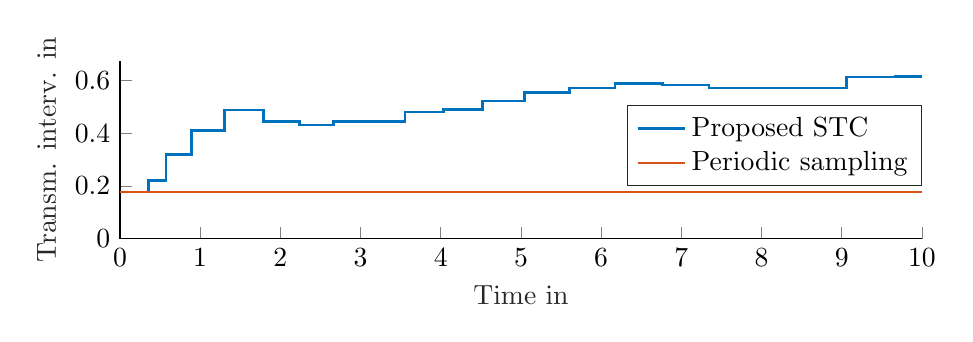
\begin{tikzpicture}

\begin{axis}[%
width=.84\linewidth,
height=.89in,
at={(0in,0in)},
scale only axis,
xmin=0,
xmax=10.0,
ymin = 0.0,
xlabel style={font=\color{white!15!black}},
xlabel={Time in \SI{}{\second}},
ylabel style={font=\color{white!15!black}},
ylabel={Transm. interv. in \SI{}{\second}},
axis background/.style={fill=white},
%
%
axis x line*=bottom,
axis y line*=left,
legend style={legend cell align=left, align=left, draw=white!15!black,at={(1,0.75)}}
]
\addplot[const plot, color=mycolor1, line width=1.0pt] table[row sep=crcr] {%
0	0.177257784781798\\
0.177257784781798	0.177257784781798\\
0.354515569563596	0.219396716821825\\
0.573912286385421	0.318966280802836\\
0.892878567188257	0.409470876897616\\
1.30234944408587	0.4881756171017\\
1.79052506118757	0.444044228823746\\
2.23456929001132	0.430741711235353\\
2.66531100124667	0.44393101538901\\
3.10924201663568	0.444044228823746\\
3.55328624545943	0.480060904901628\\
4.03334715036106	0.491071049609055\\
4.52441819997011	0.522141612224481\\
5.04655981219459	0.554735786884006\\
5.6012955990786	0.571352302216618\\
6.17264790129521	0.588622320394373\\
6.76127022168959	0.583281011304961\\
7.34455123299455	0.571352302216618\\
7.91590353521117	0.571352302216618\\
8.48725583742779	0.571352302216618\\
9.0586081396444	0.612908409606037\\
9.67151654925044	0.61381480923818\\
10.2853313584886	0.635399477042316\\
};
\addlegendentry{Proposed STC}

\addplot[const plot, color=mycolor2, line width=1.0pt] table[row sep=crcr] {%
	0	0.177257784781798\\
	11	0.177257784781798\\
};
\addlegendentry{Periodic sampling}
%
%
%
%
%
%
%
%
%
%
%
%
%
%
%
%
%
%
%
%
%
%
%
%
%
%

\end{axis}


\end{tikzpicture}%
		\vspace{-7mm}
	\caption{Time between successive transmissions for the proposed STC mechanism and periodic sampling.
		%
	}
	\label{fig_inters}
	%
\end{figure}